\documentclass{article}

\usepackage[T1]{fontenc}
\renewcommand{\ttdefault}{lmtt}
\usepackage{iclr2026_conference,times}
\usepackage{amsmath,amssymb,booktabs,array,graphicx,microtype,float,longtable}
\usepackage{tikz}
\usetikzlibrary{arrows.meta,positioning}
\usepackage[hidelinks]{hyperref}

% Keep evidence-heavy float-only appendix pages top-aligned. LaTeX otherwise centres a
% lone full-page table vertically, which created the visual-audit whitespace on Tables 5--7.
\makeatletter
\setlength{\@fptop}{0pt}
\makeatother

% Machine strings (verdicts, paths) are typeset with \path so that they may break
% after "/" and "_" inside narrow table columns instead of overflowing them.
\newcolumntype{L}[1]{>{\raggedright\arraybackslash}p{#1}}
\newcolumntype{Q}[1]{>{\scriptsize\raggedright\arraybackslash}p{#1}}

% Explicit three-line title: measured \LARGE\sc widths are 115.4pt / 374.2pt / 256.8pt
% against \textwidth=397.5pt, so no line overflows and none is hyphenated. Every
% two-line split overflows one line (breaking after "Operability" hyphenates it as
% "Oper-/ability"; breaking after "Endpoint" leaves a 416.9pt second line), which the
% page-by-page visual review of paper/layout/pages/page-001.png flagged.
\title{AUDIT-GATE:\\
A Pre-Registered, Replayable Operability Audit\\
for Multi-Agent Research Archives}

\author{Anonymous authors}

\begin{document}
\raggedbottom

\maketitle

\begin{abstract}
Multi-agent research runs leave \emph{fire archives}: pre-registrations, endpoint code,
and reports that claim a decision fired.  We present AUDIT-GATE, a static zero-GPU audit
developed during one live run, together with a transparency record of what was
pre-registered, amended after observation, preserved, or found to have drifted.  The audit
returns exactly one of PASS, FAIL, or POSTPONE.  Each verdict includes a replayable
certificate consisting of pinned inputs, a pinned checker, and one command.  This bundle is
an interface that a third party can execute; no third-party execution is claimed here.

AUDIT-GATE combines four archive checks---endpoint reachability, boxed positive controls,
manifest acceptance, and unreachable-primary-leg archiving---with a five-field endpoint
registration rule, a healthy-arm non-degeneracy criterion, and PRIM5, which projects raw
machine strings onto the three verdict states.  The field audit comprises a six-case
frozen-checker ledger and a preregistered decisive cell over seven archives from other seats
in the same run.  At the frozen auditor-transcription tier, the decisive cell contains $6$
PASS, $1$ FAIL, and $0$ POSTPONE; after mechanical extraction and current-verdict
synchronization, it contains $3$ PASS, $2$ FAIL, and $2$ POSTPONE.

The fourteen frozen field units exercise PASS and FAIL but not POSTPONE.  Eight synthetic
defect-injected archives exercise the missing state and every emitting clause; the sole
zero is the intended absence of an unregistered verdict string.  These fixtures establish
mechanical branch coverage, not detection or false-alarm performance on natural archives.
Because the run contains no independently labelled archive population, we report no such
rates and instead register the design needed to measure them.  AUDIT-GATE tests whether a
verdict is mechanically operable and replayable, not whether it is scientifically correct.
\end{abstract}

\section{Introduction}
\label{sec:intro}

A fire claim states that a preregistered decision point fired.  In a multi-agent run, the
supporting archive contains a frozen preregistration, consumer scripts, and result reports.
Three forms of drift complicate review: prose can diverge from artifacts, rerunning current
code may no longer reproduce the registered computation, and producer self-attestation need
not track the computation performed~\citep{turpin2023language}.  AUDIT-GATE addresses the
earlier, static question of whether the registered decision is mechanically reachable and
replayable.  Figure~\ref{fig:teaser} summarizes the resulting object.  Because the gate was
built inside one live run, we report post-observation amendments as part of its construction
history (Tables~\ref{tab:preregdiff} and~\ref{tab:repin}).

\begin{figure}[t]
\centering
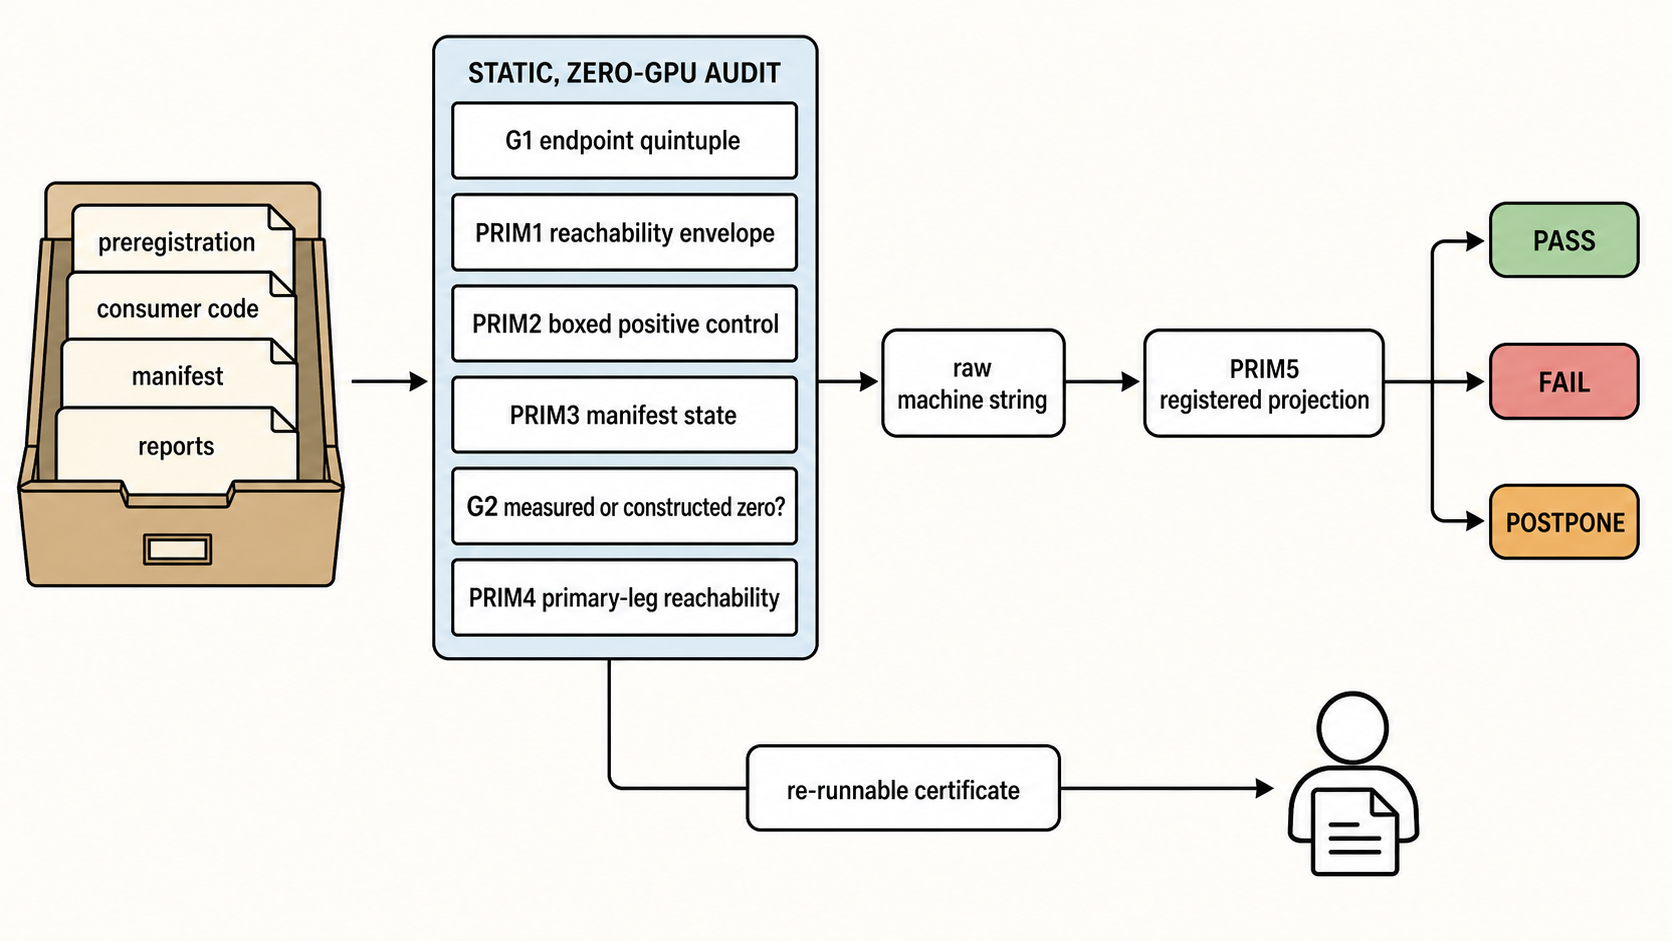
\includegraphics[width=0.98\textwidth]{figures/teaser_candidate_r44_v3.png}
\caption{The audit in one picture. A fire archive enters as files (pre-registration,
consumer scripts, manifest, reports); a fixed sequence of static checks is applied without a
GPU or a model; each check may terminate with a machine string, which a registered
projection maps onto exactly one of PASS, FAIL, POSTPONE (Section~\ref{sec:prim5}); and the
verdict ships with a re-runnable certificate --- a frozen script plus record-time anchors ---
so that an independent party can recompute it. The illustration is a qualitative schematic
produced with an image generator and audited element by element against
Section~\ref{sec:framework}; it contains no quantitative values, no data and no experimental result.
Figure~\ref{fig:pipeline} gives the same chain with each check's exact terminal verdict.}
\label{fig:teaser}
\end{figure}

Many archives fail before a statistical question is reachable: no consumer script computes
the registered readout; a rate is defined over an empty denominator; a manifest references
missing, unmarked artifacts; or a supposedly healthy zero comes from a deterministic replay
of the same path.  Detecting these conditions requires neither a GPU nor a model, only a
static inspection of the recorded files.

AUDIT-GATE maps a fire archive to PASS, FAIL, or POSTPONE using filesystem- and
string-level facts.  A verdict is reportable only with a replayable certificate: a frozen
script that recomputes it from record-time anchors.  Our contributions are:

\begin{enumerate}
\item \textbf{A meta-primitive layer} (Section~\ref{sec:framework}): four primitives
PRIM1--PRIM4, the G1 endpoint quintuple
$(\text{readout},\ \text{side},\ n,\ \text{threshold},\ \text{path\_id})$, the G2
non-degenerate-healthy-arm criterion, a disambiguation of \emph{when} a consumption
verdict is evaluated, and PRIM5, which closes the verdict domain by pinning the projection
from raw machine strings onto the three states.
\item \textbf{A re-runnable certificate discipline}: a verdict counts only if a frozen
script reproduces it and every anchor is pinned to its record-time location. The bundled
pin, checker, and one-command replay form an independent re-run interface that a third
party can execute; we do not claim that one already has. We separate record-time semantics
from today's write-time re-pinning and disclose every disagreement.
\item \textbf{A two-ledger field audit} (Section~\ref{sec:results}): a six-case ledger
over real in-run fire archives, plus a decisive cell whose pre-registration was frozen
before it ran and which replays the audit over seven external archives, including one
true detection and one deliberate non-kill. Because the live corpus turned out to exercise
only two of the three states, we add eight synthetic defect-injected archives that exercise
the third and close the anchor enumeration (Section~\ref{sec:fixtures}), and we report the
resulting coverage gap explicitly rather than describing the observed verdict set as
non-vacuous.
\end{enumerate}

Two framing clauses hold throughout. Mechanical operability is not empirical soundness: a
PASS may still be statistically wrong, and we make no claim about an archive's science.
The verdict map, PRIM3 enumeration, G2 predicate, and tier reading changed after
observation; we disclose these changes rather than pretending the current shape was
pre-registered. Appendix~\ref{app:pin} is the single current-verdict statement.

\section{Framework}
\label{sec:framework}

\paragraph{Objects.}
A fire archive $A$ consists of a pre-registration, a set of consumer scripts $C(A)$ that
are supposed to compute the registered reading, a manifest $M(A)$ of referenced
artifacts, and reports. The audit target is not the reading but the \emph{verdict}: can a
second machine, given only $A$ as it was recorded, recompute the same three-state
outcome? Figure~\ref{fig:pipeline} fixes the order in which the checks of this section are
applied and names the terminal verdict each one may emit.

\subsection{G1: the endpoint quintuple}
\label{sec:g1}

Every registered endpoint must be pinned as
\[
e = (\text{readout},\ \text{side},\ n,\ \text{threshold},\ \text{path\_id}),
\]
and a missing field returns POSTPONE with the minimal refill, never a bare ``insufficient
sample''. Thresholds are meaningful only within one \texttt{path\_id}; cross-path
differences are outside that endpoint's calibration. Appendix~\ref{app:g1} gives the full
path identity and the decisive cell's per-unit registrations.

\subsection{PRIM1--PRIM4}
\label{sec:prims}

\textbf{PRIM1 (reachability envelope).} The endpoint side, readout, and $n$ must be pinned.
Let $[L,U]$ be the two-sided $95\%$ Clopper--Pearson interval~\citep{clopper1934use} for
$k$ successes in $n$ trials at $\alpha=0.05$, and let $\theta$ be the registered threshold.
An endpoint is \emph{design-decidable} when at its registered $n$ some observable outcome
either crosses $\theta$ or certifies equivalence, and \emph{observed-decided} when the
observed interval actually does so:
\[
\textsc{lo}:\ U \le \theta;
\qquad
\textsc{hi}:\ L \ge \theta;
\qquad
\textsc{abs}\ (\text{TOST}):\ [L,U]\subseteq[\theta-\delta,\theta+\delta]
\]
for a pre-registered margin $\delta>0$. The retired singleton-intersection reading
$[L,U]\cap\{\theta\}$ trivialized at $n=1$: it made every such endpoint automatically
``decided.'' Under TOST, $n=1$ is never automatically observed-decided, and an unregistered
$\delta$ is a post-hoc zone. An interval satisfying no branch yields POSTPONE with a
minimal-refill obligation. For the degenerate zero column $k=0$,
\[
U(n) \;=\; 1-\Bigl(\tfrac{\alpha}{2}\Bigr)^{1/n},
\]
so the refill is the integer
$n^{\star} = \min\{\, n : U(n) \le \theta \,\}$. The exercised numeric instance and its
checked refill are reported in Table~\ref{tab:fixtures} (PTSD-2); the runner recomputes
$n^{\star}$ by search rather than reciting it.

\textbf{PRIM2 (boxed positive control).} Every gate must carry at least one must-FAIL arm
built from a known-illegal input, boxed away from the primary data, with the acceptance
criterion that the must-FAIL arm fires on all of its cases while the anti-pass arm fires
on none. A positive control that passes unconditionally has zero evidential strength, and
the audit reports FAIL rather than a passing gate.

\textbf{PRIM3 (manifest three-arm acceptance).} For every artifact referenced by a
manifest, exactly one of three arms applies: present with matching hash (PASS); present
with drifted hash and no recorded cause (FAIL); \emph{absent without an explicit ABSENT
marker} (FAIL). The third arm is the one that produced this framework's own constructive
self-FAIL, case F3 of Section~\ref{sec:leg1}; we make no claim that it is the most productive
arm, because in our corpus no detecting arm fired more than once (Figure~\ref{fig:coverage}).
These three arms are
the states the field corpus produced; the decision is really a function of four record-time
facts, and Section~\ref{sec:fixtures} closes the enumeration at five states, adding
drift-with-a-recorded-cause (PASS) and absent-with-a-marker (POSTPONE).

\textbf{PRIM4 (unreachable primary leg).} If the primary leg's self-test corpus is
unreachable in the round being claimed --- zero scorable rows, empty manifest --- the
negative-result archiving verdict holds automatically, and re-labelling the failed primary
run as a sensitivity analysis is forbidden.

\subsection{G2: was the zero measured or constructed?}
\label{sec:g2}

Gates that calibrate on ``the healthy arm shows zero false alarms'' must distinguish a
measured zero from a constructed one. A deterministic or zero-dispersion healthy arm carries
no threshold information, so the audit emits \path{FAIL_DEGENERATE_HEALTHY_ANCHOR}. The
current runner earns that verdict from the archived fields rather than assigning it as the
superseded edition did (Table~\ref{tab:preregdiff}). Its same-path probe is an
\texttt{r42} snapshot, not an invariant floor. A threshold may be repaired before freezing;
changing it after observation is a gate swap.

\subsection{Where the consumption verdict is evaluated}
\label{sec:binding}

A recurring ambiguity is when to judge that a primitive was consumed. We bind the
evaluation to the producer's own pre-registered binding decision point, then to the later
of (the consumer's first consuming round, the producer's release round), plus $K$ observer
rounds with $K=2$ by default. This single rule excludes the two opposite readings that
otherwise coexist: ``any action by any seat counts as consumption'' and ``only the
producing seat's actions count''.

\subsection{Advisory status, disclosed in full}
\label{sec:advisory}

The fan-in ledger that records consumption evidence carries the structural property
\path{cannot_FAIL_by_design}${}={}$\path{true}, and we keep that disclosure in the main
text rather than in a footnote. Its meaning is narrow and must not be inflated in either
direction: the ledger never auto-promotes itself to a mandatory gate, which is not the same
as never emitting FAIL. It does emit FAIL verdicts, and the two on record are a constructive
self-FAIL on this framework's own ledger (four of five recorded consumer paths absent at
their recorded locations without ABSENT markers) and a reusable counterfactual template any
seat can apply post hoc. A scoreboard is not a gate; we report it as advisory evidence, never
as a blocking condition on another seat.

\subsection{What ``mechanically operable'' means}
\label{sec:operable}

A verdict is mechanically operable when (a) it follows from filesystem- or string-level
facts, (b) a re-runnable script certificate recomputes it, and (c) every anchor is pinned
to the artifact's location \emph{at the time of record}. Condition (c) is not pedantry: an
early version of our own audit resolved an anchor to where the file would be looked up
later, and a failure to reproduce at that later path is a stale anchor, not a falsified
original verdict.

\paragraph{Freeze-discipline disclosure.}
The first-run implementation contradicted the registered diversity predicate and returned
\path{FAIL_VACUOUS_STATES}; it was corrected only after observing the cell. Worse, that
edition was replaced before it was pinned, so the verdict is recorded but not recomputable.
By our own PRIM3 and certificate rule this is a \emph{self-FAIL of our record-keeping}, not a
repairable footnote. The verdict-state map, PRIM3 enumeration, and G2 predicate also changed
after observation. Table~\ref{tab:preregdiff} and Appendix~\ref{app:statemap} preserve the
version-by-version account, including the record-time/write-time distinction.

\subsection{PRIM5: verdict-domain closure}
\label{sec:prim5}

Checkers emit reason-bearing machine strings, not states. PRIM5 therefore registers a map
from every emitted string onto exactly one of PASS, FAIL, or POSTPONE and applies it by
script. Provenance prefixes are stripped; an absent string becomes \path{UNMAPPED} and makes
the certificate fail; unit and group strings occupy separate codomains; and each entry says
how it was exercised. The complete rules and map are in Appendix~\ref{app:statemap}; the
projection command is in Appendix~\ref{app:repro}.

\paragraph{What a group verdict does and does not assert.}
The decisive cell's group verdict is about audit execution, not a conjunction over archive
verdicts: it says the audit ran, mapped every string, exercised its controls, and separated
at least two projected states. Its canonical machine string is
\path{EXECUTION_VALID} (renamed from \path{AUDIT_EXECUTION_PASS} so the label cannot be
misread as archive operability). Panel~B of Table~\ref{tab:ledger} separately reports archive
operability and includes a FAIL; Appendix~\ref{app:statemap} preserves the rule and its
bidirectional disagreements.

\section{Field audit}
\label{sec:results}

We report a six-archive ledger audited in place and a decisive cell, frozen before it ran,
over seven external archives owned by other seats. Table~\ref{tab:ledger} carries both.
Seat identities are anonymized throughout: unit keys lead with owner-seat letters A--H,
and neighbour assets are cited by role and sha16, never by per-seat filesystem paths.

At the frozen tier, the live corpus occupies only PASS and FAIL and never POSTPONE. Thus
PRIM1's non-crossing envelope and PRIM4's unreachable primary leg have empty live cells.
We do not call that set non-vacuous; Section~\ref{sec:fixtures} exercises the missing state
on built-for-purpose archives and preserves the live-corpus POSTPONE count of zero.

\subsection{Leg 1: six-case ledger}
\label{sec:leg1}

Panel~A of Table~\ref{tab:ledger} is the ledger frozen at R27
(\path{analysis/AUDIT_LEDGER_R27.json}, sha16 \path{64bf94507159fec4}), with the r29
amendment that finalises case F5 and the R30 amendment that pins the repair-shape lineage
discussed in Section~\ref{sec:related}. The headline result of this leg is a reproduction
property rather than a measurement: \emph{all six ledger verdicts, plus the lineage arm,
are reproduced by the frozen checker on the current disk state}
(\path{analysis/audit_gate.py}, sha16 \path{0ed8657a6ab7dbf9}, exit code $0$;
Appendix~\ref{app:repro} gives the exact invocation). The failure modes in the panel are
distinct from one another, one per primitive, and the Reason column states each in one
line. F4 is the panel's positive control, an archive that an independent audit had already
examined line by line and which our framework does not false-kill (it is judged operable
and we do not kill it; Section~\ref{sec:falsification}). F6 is the one
system-level case: two lifecycle
transition branches coexist such that a single submission can telescope two stage
transitions, which is a property of source text rather than of data.

Two provenance notes belong in the main text. The r29 amendment recorded the checker at
sha16 \path{1e88186f7097646b}; the current sha16 differs because the R30 amendment added
the read-only lineage arm, and the six case verdicts are unchanged by that arm. And F5's
final verdict asserts only that the fire archive landed with an authorisation chain and a
resolvable anchor. It does not re-adjudicate the audited seat's statistical conclusion,
which remains that seat's own claim.

\subsection{Leg 2: pre-registered decisive cell}
\label{sec:leg2}

Panel~B is the decisive cell D1 (pre-registration
\path{experiments/prereg/PREREG_AUDIT_GATE_D1.md}, sha16 \path{7a2d5306b734478f}; runner
\path{code/run_audit_gate_d1.py}, sha16 \path{88922152856c9e98}). The cell was registered so
that non-recomputable verdicts or a collapsed verdict set would fail. It returned
\emph{group verdict PASS} in the audit-execution sense of Section~\ref{sec:prim5}; the frozen
and current judge tiers remain separate below.

The \emph{frozen tier} is the registered R31 report (sha16
\path{d91f180ea59edc39}); its projection regenerates byte-identically (sha16
\path{aba51fa7f7b3a8b9}) and supplies Panel~B. Its stronger pre-registered byte-identity
branch is no longer met: current sidecars are deterministic, but differ from the frozen
report because one live audited archive and the judge edition drifted. We therefore record
that branch as fired and retain only the tier-specific verdict-recomputation claim.

The repaired R42 judge initially agreed with the frozen tier on every unit. A later replay
changes the seat-E unit from PASS to FAIL, and the R52 mechanical extractor makes the
previously transcribed G2 answer for seat C and threshold for seat H unavailable, so they
POSTPONE under G1's rule. Thus the current tally is $3$ PASS, $2$ FAIL, $2$ POSTPONE while
the frozen tally remains $6$ PASS, $1$ FAIL, $0$ POSTPONE. This is archive/provenance drift,
not runner nondeterminism (Section~\ref{sec:replay}).

The cell contains one true detection and one deliberate non-kill. The detection is the
same-path unit, where G2 fires because the healthy arm's zero is constructed --- in the
current tier that verdict is earned by the predicate reading the audited cell's own
\texttt{bit\_exact=true} and \texttt{max\_max=0.0} fields (\texttt{code/run\_audit\_gate\_d1.py},
\texttt{audit\_p6}; in the frozen tier it was, as an external review made us discover, an
unconditional assignment, which is row four of Table~\ref{tab:preregdiff}). The non-kill
is the perturbation-smoke unit, whose owner self-reports a thin margin on easy prompts: a
thin margin is a covariate of that seat's experiment, not an operability defect, and the
audit does not convert it into a FAIL. The framework also self-FAILed once, on its own group
gate; because that correction happened after the observation, we report it as a
pre-registration diff rather than as an anecdote, under the freeze rule
(Section~\ref{sec:operable}, Table~\ref{tab:preregdiff}). A verdict channel that cannot fail
on itself is exactly the object this framework refuses to accept from others, so the
correction is disclosed rather than smoothed away.

\begin{table}[t]
\caption{Two-leg field audit. \textbf{Panel A}: the six-case ledger plus the A4
amendment, at its frozen-ledger tier. \textbf{Panel B}: decisive cell D1 over seven external
fire archives, printed at the frozen auditor-transcription tier. Across both panels the
$14$ exact machine outputs project to $9$ PASS, $5$ FAIL and $0$ POSTPONE. The current
mechanical tier is separate: $3$ PASS, $2$ FAIL and $2$ POSTPONE
(Appendix~\ref{app:pin}). The starred unit is the positive control; the daggered seat-E
unit changes from frozen PASS to current FAIL. The registered map is
Appendix~\ref{app:statemap}; commands and sha16 anchors are Appendices~\ref{app:repro}
and~\ref{app:anchors}.}
\label{tab:ledger}
\centering
\scriptsize
\setlength{\tabcolsep}{3pt}
% Verdict column is 78pt because the widest \path fragment that must sit on one line,
% "FAIL_MECHANICALLY_" / "EXTERNAL_CANDIDATE", measures 75.6pt at \scriptsize; at the
% earlier 74pt both verdicts spilled onto a third line. Case is 82pt so that every
% Panel B unit key (widest, C_exit_package_R42, is 79.5pt) stays on one scannable line.
% Folding the redundant State column into the tally gives its width to Reason.
\begin{tabular}{@{}L{82pt} L{50pt} L{78pt} L{112pt} L{50pt}@{}}
\toprule
Case & Fire archive & Verdict (machine string) & Reason & Replayer \\
\midrule
\multicolumn{5}{@{}l}{\emph{Panel A: six-case ledger (R27, amended r29 and R30)}}\\
\addlinespace[1pt]
F1 & quant-gate prereg (seat G) & \path{FAIL_MECHANICALLY_UNREACHABLE}
   & registered reading has no computor in any of the three consumer scripts
   & external, 3 sha16 \\
F2 & legacy post-create gate (seat D) & \path{FAIL_EMPTY_SET_PASSED_GATE}
   & empty denominator falls back to a passing rate & owner post-mortem \\
F3 & own fan-in ledger (self-audit) & \path{FAIL_ABSENT_UNMARKED_4_OF_5}
   & recorded consumer paths absent, no ABSENT marker & constructive self-FAIL \\
F4 & four-closure prereg (seat C) & \path{PASS_OPERATIONAL}
   & all computors present; bound is a computed number & external line audit \\
F5 & two-cell rerun archive (seat G) & \path{__r29_pin__FINAL_FIRE_LANDED}
   & landed with authorisation chain; anchor resolves & amendment pointer \\
F6 & lifecycle stage gate (harness) & \path{FAIL_TELESCOPE}
   & two transition branches coexist in one submission & source signature \\
A4 & readout health gate (seat D, amendment)
   & \path{PASS_OPERATIONAL_EXTERNAL_CANDIDATE}
   & positive arm passes while the dead-parser arm fails & four pinned sha16 \\
\addlinespace[2pt]
\midrule
\multicolumn{5}{@{}l}{\emph{Panel B: decisive cell D1 (R31), seven external fire archives;
projected-state tally $6$ PASS, $1$ FAIL, $0$ POSTPONE}}\\
\addlinespace[1pt]
\path{D_A4_healthgate}$^\star$ & readout health gate & \path{PASS}
   & positive control: gate passes while its fail arm decouples & frozen runner \\
\path{C_exit_package_R42} & refine exit package & \path{PASS}
   & every registered issue slot carries a resolved mark, per a registered slot manifest
     (\texttt{audit\_p3}) & frozen runner \\
\path{E_R33_threearm}$^\dagger$ & three-arm calibration & \path{PASS}
   & registered bound and an explicit three-arm design present in the archive
     & frozen runner \\
\path{F_r42_samepath} & same-path certificate
   & \path{FAIL_DEGENERATE_HEALTHY_ANCHOR}
   & constructed-zero healthy arm (current tier: predicate over the cell's own
     \texttt{bit\_exact}${}={}$true, \texttt{max\_max}${}={}0$); threshold anchored by the
     mismatched-path arm alone
   & frozen runner \\
\path{G_fb2_v3_r120} & authorised rerun verdict & \path{PASS}
   & verdict keywords and trial id in the verdict file, spec name pinned in the job
     file & frozen runner \\
\path{H_r7_conject_front} & perturbation smoke & \path{PASS}
   & required arm present at pinned $n$; thin margin is a covariate & frozen runner \\
\path{A_r7_strict_corpus} & strict-corpus gate & \path{PASS}
   & coverage rows measured from the real corpus & frozen runner \\
\bottomrule
\end{tabular}
\end{table}

\subsection{Synthetic defect-injected fixtures for the unexercised state}
\label{sec:fixtures}

Because the live corpus never exercised POSTPONE or several primitive branches, we wrote
defect-injected fire archives in the style of mutation testing~\citep{jia2011analysis}. Each
fixture injects one registered defect; the runner recomputes its verdict and refill rather
than reading an expected answer, and all rows match without a GPU. Table~\ref{tab:fixtures}
and Appendix~\ref{app:fixtures} give the complete per-fixture record and PRIM3 enumeration.

\paragraph{Where each check was exercised, and where it was not.}
Figure~\ref{fig:coverage} derives the live-versus-fixture ledger from registered artifacts,
including its zeros. It shows exactly which checks depend on authored fixtures and which
live branches were never evaluated; the PRIM5 unmapped-string zero is the intended reading,
because any fire would break the certificate.

\begin{figure}[t]
\centering
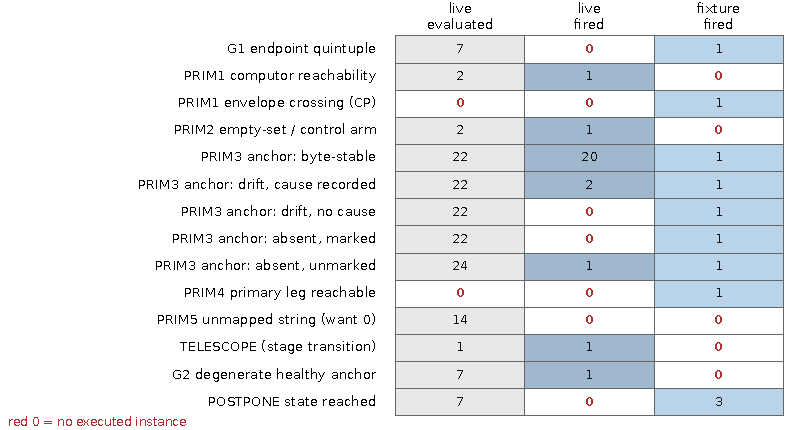
\includegraphics[width=\textwidth]{figures/fig_coverage_matrix.pdf}
\caption{Where each check of the framework was exercised, computed from on-disk artifacts by
\texttt{make\_coverage\_matrix.py} (Appendix~\ref{app:repro}). \emph{Live evaluated} counts the
units or ledger arms on which the check actually ran; \emph{live fired} counts those where its
detecting branch was taken; \emph{fixture fired} counts the synthetic archives of
Section~\ref{sec:fixtures}. Zeros are printed in red and in the same weight as the counts,
because they are this note's own admissions rather than blanks: a red zero in the live column
of the PRIM1 envelope row says the field corpus never exercised that clause. The one row that
is zero in both fire columns is PRIM5's unmapped-string counter, and there zero is the intended
outcome --- an unregistered verdict string would break the certificate by design.}
\label{fig:coverage}
\end{figure}

Two limits of this evidence should be read with it. These fixtures demonstrate that the
POSTPONE, PRIM4 and anchor-state clauses are \emph{mechanically operable} --- they fire on
inputs constructed to trigger them and they return the refill obligation the specification
promises --- and they do not demonstrate detection performance on natural archives, because we
authored both the defect and the checker. They are positive controls in the sense of PRIM2,
not a calibration; the missing calibration is still missing, and
Section~\ref{sec:falsification} says so.

\subsection{Replaying the certificates at writing time}
\label{sec:replay}

Both certificates were replayed while writing. Every ledger arm reproduces; the decisive
cell retains its group PASS, but only six of the seven frozen unit verdicts do. The changed
unit audits a live external manuscript whose current text no longer satisfies its registered
predicate. Table~\ref{tab:anchortally} is the earlier all-unit-stable snapshot; the current
divergence, negative controls, figure, and commands are in Appendix~\ref{app:repro}.

\section{Related work}
\label{sec:related}

\paragraph{The nearest in-run neighbour, and why it is complementary.}
The closest artifact is a killed seat's readout health gate and its anti-patterns. We reuse
rather than rebuild them: that gate tests empirical readout correctness, whereas ours tests
the mechanical operability of a registered decision. Table~\ref{tab:delta} gives the main
axes; Appendix~\ref{app:delta} gives the rest.

\paragraph{Other in-run primitives.}
A post-create assertion script gates artifacts immediately, whereas PRIM3 audits later
manifests; an in-run reachability checklist belongs to PRIM1's family and is a merge
candidate, not a baseline.

\paragraph{External lineage: two classical ancestors.}
Clopper--Pearson intervals supply PRIM1's envelope~\citep{clopper1934use}; statistical
process control supplies the principle that a gate's authority comes from calibration, not
operator judgement~\citep{shewhart1931economic}.

\paragraph{External positioning: three literatures this is not.}
Provenance and experiment-lineage systems record how values and models were produced
\citep{cheney2009provenance,vartak2016modeldb,schelter2017automatically,zaharia2018accelerating},
while versioning pins their artifacts~\citep{kuprieiev2020dvc}; AUDIT-GATE instead asks
whether a claimed adjudication is recomputable. Reporting standards and preregistration
govern author-side disclosure~\citep{pineau2021improving,gebru2021datasheets,forde2019scientific},
and production assertions inspect data or model behaviour in flight
\citep{polyzotis2019data,kang2020model}; our audit acts later on a released archive.
Content-addressed deployment and reproducible builds establish byte identity
\citep{dolstra2004nix,lamb2022reproducible}; PRIM3 additionally distinguishes explained drift
from absence because its target is verdict stability. If these deltas amount only to MLOps
governance common sense, the registered MERGE clause requires folding the framework into a
survey and retiring it.

\begin{table}[t]
\caption{Delineation from the nearest in-run neighbour (three of five axes; the remaining
two are in Appendix~\ref{app:delta}).}
\label{tab:delta}
\centering
\scriptsize
\setlength{\tabcolsep}{4pt}
\begin{tabular}{@{}L{58pt} L{158pt} L{158pt}@{}}
\toprule
Axis & Readout health gate (neighbour) & AUDIT-GATE (this note) \\
\midrule
D1 audited object & empirical correctness of a readout: does the parser or grader work on
real model output? & mechanical operability of a registered decision point: does the
registered reading have a computor, an envelope, a fireable control? \\
\addlinespace[2pt]
D2 work phase & before a run: positive, negative and length controls on the data the run
will consume & before creation (static reachability) \emph{and} in any later round
(post-hoc manifest three-arm acceptance) \\
\addlinespace[2pt]
D3 formalisation & thresholded empirical checks with a binary outcome & envelope plus
boxed control injection with an explicit three-state outcome; the binary gate is its
degenerate case \\
\bottomrule
\end{tabular}
\end{table}

\section{Falsification and scope}
\label{sec:falsification}

The four registered exits remain. \textbf{PASS} is a population-level aspiration: all
mechanically unreachable endpoints are caught (false-open ${}={}0$) and no operable archive
is killed (false-kill ${}={}0$); a finite corpus can certify only bounds on those rates.
\textbf{KILL} fires if an independently confirmed unreachable endpoint is judged PASS or
the false-kill rate is evidenced above $5\%$. \textbf{MERGE} withdraws the framework into a
survey if it merely restates MLOps governance. \textbf{STOP-PASS} additionally requires one
independent external fire claim to adopt the primitives as its pre-creation gate.

Two further candidates came from in-run review (Appendix~\ref{app:delta}). Clause (vii) is
falsified by a gate that reaches its registered bound, has no post-hoc discriminating power,
and is not rejected by (viii). Clause (viii) is falsified by byte-identical load-bearing
fields that do not make a downstream paired or maximum comparison tautological.

Two scope limits follow. A PASS means recomputable, not scientifically correct. Nor do we
calibrate the audit's false-alarm rate or power: the fixtures do not close this gap because
they share an author with their checkers. Calibration requires a labelled fire-archive
population whose operability status is established independently of us, which does not
exist inside a live run.

Mitigation (i) is an author-withheld-label blind calibration over $8$ frozen fixture labels: a blind wrapper reproduced a diagonal confusion matrix and reports two-sided Clopper--Pearson bounds (\path{analysis/r83_i22_calib/I22_BLIND_CALIBRATION_R83.json}); because the fixtures and checker share an author, this is a mitigation, not calibration closure, and it is not third-party execution. Mitigation (ii) is a clean-room bundle with single-entry \path{replay.py}, a hash-first-frozen \path{MANIFEST}, and a self-test reporting \path{replay_pass=true} (\path{experiments/bundle_i21_r83.tar.gz}); it is a mitigation, not calibration closure, and it is not third-party execution. Together they make label visibility and replay packaging auditable while leaving the missing independent population and third-party run unresolved.

What is available is the design that would settle the question, registered before any
number exists. The v1 cell is superseded before execution; the v2 cell is \emph{blocked},
not merely unrun: it needs at least $118$ independently labelled defect-free archives, and
unblocks only with a labeller outside the authoring seat, an outcome that remains
human{\_}pending. Table~\ref{tab:calibration-summary} records the decisive inequalities;
\path{analysis/D2_DECISION_REACHABILITY_R52.json} verifies a total, single-valued outcome
map.

\begin{table}[!t]
\caption{Registered calibration-cell decision design. The v1 acceptance region cannot
decide the manuscript's $5\%$ false-kill boundary; the v2 repair is decisive on that
boundary. The v2 cell is \emph{blocked}, not merely unrun: it requires at least $118$
independently labelled defect-free archives and a labeller outside the authoring seat
(human{\_}pending).}
\label{tab:calibration-summary}
\centering
\small
\setlength{\tabcolsep}{3pt}
\begin{tabular}{@{}L{82pt} L{145pt} L{145pt}@{}}
\toprule
Design item & v1 registration & v2 registered repair \\
\midrule
False-kill cell & $n=60$; accept at most one fire; $0.10$ upper-bound rule
  & $n=118$; accept at most one fire; unified $0.05$ target \\
Decisive bound & $\operatorname{upper}(0/60)=0.0596>0.05$; even zero fires misses
  & $\operatorname{upper}(1/118)=0.0463<0.05$; largest accepted count meets target \\
Outcome map & registered acceptance region cannot decide the target
  & all $7140$ compositions are total and single-valued; no accepted composition violates $5\%$ \\
Detection side & \multicolumn{2}{L{296pt}@{}}{shared registered criterion: $36/36$ per family; lower bound $0.9026>0.90$} \\
\bottomrule
\end{tabular}
\end{table}

\section{Open items and conclusion}
\label{sec:open}

The exit ledger remains unresolved.  PASS is unmet because no independent-operability
denominator supports universal zero-miss or false-kill language.  KILL is not triggered,
but its false-kill arm is uncomputable; MERGE remains open; and STOP-PASS is unmet because
no external fire claim adopted the primitives as a pre-creation gate.

The framework, ledgers, decisive cell, and fixtures are static and GPU-free; lifetime GPU
consumption is zero.  The R42 and R52 records establish process independence, not party
independence: both ran in the same workspace, filesystem, and seat credentials.  The R83
clean-room bundle makes the replay interface portable and self-checking, but no third party
has executed it.  Appendix~\ref{app:repro} gives the commands and
Appendix~\ref{app:pin} the attested pin.

Finally, an automated writing engine revised this manuscript and an image generator produced
Figure~\ref{fig:teaser}; the figure is qualitative, and all quantitative content remains
artifact-derived. Build, prompt, semantic-audit, and authorship provenance are retained in
the accompanying ledgers.

The resulting contribution is therefore a replayable operability audit with an explicit
construction history and calibration gap, not a validated classifier of scientific quality.

% P5_MAIN_TEXT_END
\label{p5:main-text-end}
\bibliographystyle{iclr2026_conference}
\bibliography{refs}

\appendix

\section{Reproduction commands}
\label{app:repro}

All sixteen command lines are read-only with respect to audited archives, require no GPU,
and run on CPU in seconds. Paths are relative to this workspace; neighbour-seat inputs use
role labels. Fourteen lines are certificates, one composes them, and one re-hashes every
sha16 literal and rejects residual publication placeholders. The five field-audit commands
follow; Table~\ref{tab:repro} lists the remaining R41 certificates, and the R52 additions
appear before the single entry point. Independent-process records cover the R42 eleven-
certificate edition and the R52 current chain; neither is party-independent.

\paragraph{Six-case ledger certificate (Panel~A).}
\begin{quote}\scriptsize\ttfamily
python3 analysis/audit\_gate.py -{}-a4-verify \textbackslash\\
\hspace*{1em}-{}-f5-yaml 'OWNER\_SEAT\_G\_WORKSPACE/experiments/'\textbackslash\\
\hspace*{3em}'qgate\_tailturnover/qs/p7\_qgate\_dec\_r1\_fb2\_v2.yaml' \textbackslash\\
\hspace*{1em}-{}-f5-spec-name p7-qgate-dec-r1-fb2-v2-r120-mgr \textbackslash\\
\hspace*{1em}-{}-f5-expected \_\_r29\_pin\_\_FINAL\_FIRE\_LANDED
\end{quote}
Expected: one \path{[OK]} line per ledger case plus one for the lineage arm, and exit
code $0$. A \path{MISMATCH} line means either that the audited archive changed or that the
ledger is stale; by PRIM3 the second case is itself a self-FAIL of this ledger.

\paragraph{Decisive cell (Panel~B).}
\begin{quote}\scriptsize\ttfamily
./run\_audit\_gate\_d1.sh
\end{quote}
Expected: \path{group_verdict=PASS} with the per-unit verdicts of Panel~B. The runner only
reads the audited archives and only writes inside its own results directory. One point of
this is load-bearing for Section~\ref{sec:operable} and we state it exactly: a re-run
re-pins every audited artifact at its \emph{current} hash, but it writes those fresh pins
into the sidecar \path{audit_gate_d1_report_current.json} and never into the frozen report,
whose bytes the recorded verdicts are anchored to. So the two files are meant to differ once
an audited archive changes, and comparing them is a measurement of the audited archives
rather than of the runner (Section~\ref{sec:replay}). The frozen report is read-only history;
if a re-run ever alters it, that is a defect in the runner, and one such defect occurred and
was rolled back in this round (Table~\ref{tab:repin}).

\paragraph{Verdict-state projection (Table~\ref{tab:ledger}; registered map).}
\begin{quote}\scriptsize\ttfamily
python3 code/project\_verdict\_states.py
\end{quote}
Expected: \path{audit_gate_d1_report_projected_r41.json} beside the frozen report, every unit
carrying a \path{state_verdict}, an empty \path{unmapped} list, and exit code $0$. The script
reads the frozen report and the registered map and writes only the projected sidecar. A
non-empty \path{unmapped} list, and the resulting non-zero exit, is the PRIM5 enforcement
mechanism of Section~\ref{sec:prim5}.

\paragraph{Synthetic fixtures (Table~\ref{tab:fixtures}).}
\begin{quote}\scriptsize\ttfamily
python3 code/audit\_gate\_fixtures.py
\end{quote}
Expected: eight \path{[OK]} lines, \path{all_match: true} in
\path{analysis/FIXTURE_RESULTS_R41.json}, and exit code $0$. The fixtures are the only
archives in this note that we authored ourselves; the runner reads no external archive.

\paragraph{Write-time replay matrix (Figure~\ref{fig:replay}).}
\begin{quote}\scriptsize\ttfamily
python3 code/make\_replay\_matrix.py
\end{quote}
Expected: \path{analysis/REPLAY_MATRIX_R33.json} with the per-unit pin classification, and
the figure source PDF. This script re-hashes pinned artifacts and re-runs the six-case
certificate; it never writes into an audited archive.

\paragraph{Write-time interpretation and record-time verification.}
Byte identity belongs to frozen inputs, whereas the audited seats continued working. A
write-time re-pin therefore locates and hashes today's files without re-adjudicating the
recorded verdict. All ledger arms reproduce. At the R41 snapshot, all decisive-cell unit
verdicts also reproduced; the latest replay instead changes the external live-manuscript
unit while retaining the group PASS. The certificate check compares current bytes against
record-time pins without replacing them, using \path{code/verify_certificate.py}.

\begin{table}[t]
\caption{Certificate reading against the cell's $22$ record-time pins, preserved as the
R41 historical snapshot: at R41 all $7/7$ unit verdicts recomputed unchanged. The current
divergence is stated immediately below; \texttt{code/verify\_certificate.py} attests only
the canonical pin of Appendix~\ref{app:pin}. Counts: \texttt{analysis/REPLAY\_LOG\_R41.json}.}
\label{tab:anchortally}
\centering
\small
\setlength{\tabcolsep}{8pt}
\begin{tabular}{@{}lc@{}}
\toprule
Reading & Count \\
\midrule
Byte-stable & $20$ \\
Drift with registered cause & $2$ \\
\bottomrule
\end{tabular}
\end{table}

\paragraph{Snapshot caveat.}
Table~\ref{tab:anchortally} is preserved byte-for-byte as the R41 record it reports. The R49
replay still returns the same anchor tally and both negative controls, but its verdict-level
check is no longer all-unit stable: \path{E_R33_threearm} changes from frozen PASS to current
FAIL after the external seat-E manuscript ceased to contain the registered three-arm predicate.
The other frozen unit verdicts and the group PASS reproduce. The machine record is
\path{analysis/CERT_VERIFY_R41.json}; this later divergence supersedes only the caption's
present-tense reading, not its historical snapshot.

The drifted manuscript and PDF carry registered causes, so the certificate reads ``anchors
drift, explained'' rather than byte-verified. A copied-anchor mutation without a cause emits
\path{FAIL_ANCHOR_DRIFT_UNEXPLAINED}; adding a fabricated cause converts it to
\path{PASS_ANCHOR_DRIFT_EXPLAINED}. Thus explained drift is only as trustworthy as its cause
registry, and a reviewer may ignore that registry and read both drifted pins as unexplained
FAILs. A second implementation agrees with the shipped checks, but remains an internal
consistency check because one author wrote both.

\begin{figure}[t]
\centering
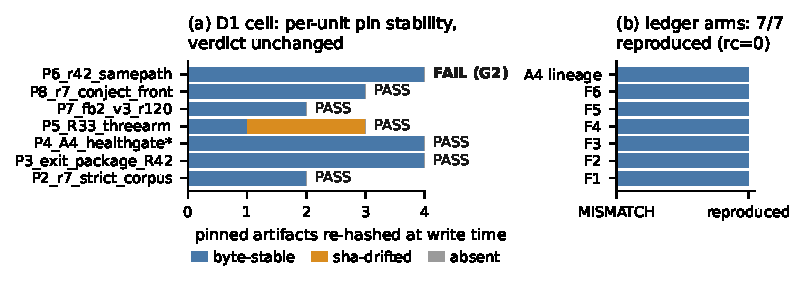
\includegraphics[width=\textwidth]{figures/fig_replay_matrix.pdf}
\caption{Write-time replay of both certificates, computed from on-disk artifacts by the
script \texttt{make\_replay\_matrix.py} (Appendix~\ref{app:repro}). \textbf{(a)} For each
unit of the decisive cell,
the artifacts pinned in the frozen report are re-hashed and classified as byte-stable,
sha-drifted or absent; the verdict recorded in the frozen report is annotated at the
right as a frozen-tier reading (not the current tier: seat E is currently FAIL), with the
one G2 verdict shortened to \texttt{FAIL}~(G2) --- its exact string is the
Panel~B row of Table~\ref{tab:ledger}. \textbf{(b)} The six ledger cases plus the lineage
arm, as reported by the re-run six-case certificate (exit code $0$). Unit labels are the
keys of the frozen report; the starred unit is the cell's positive control.}
\label{fig:replay}
\end{figure}

\paragraph{The remaining certificates.}
Table~\ref{tab:repro} lists them with the artifact each writes and the property a reviewer
should check in it. Each is one line, each reads only files inside this workspace, and each
exits non-zero when its own registered expectation fails.

\begin{table}[htbp]
\caption{The remaining commands, their artifacts, and what to check. The first six are
certificates and are included in the single entry point below; the last is a
manuscript-level check and is deliberately excluded from it, because its input is this
\texttt{.tex} file rather than the audit. The certificate verifier attests the canonical
pin of Appendix~\ref{app:pin}; it does not certify that current archive verdicts equal the
frozen tier.}
\label{tab:repro}
\centering
\scriptsize
\setlength{\tabcolsep}{4pt}
% Command column is 128pt: the longest command, code/audit_gate_second_impl.py, needs ~126pt
% at \scriptsize and broke after the final "." at 118pt in the page-by-page review. The three
% widths plus the two 8pt intercolumn gaps must stay under \textwidth=397.5pt, so the width
% comes out of the last column (128+104+149+16 = 397pt).
\begin{tabular}{@{}L{128pt} L{104pt} L{149pt}@{}}
\toprule
Command (prefix \texttt{python3}) & Writes & What a reviewer checks \\
\midrule
\path{code/make_prim3_fixtures.py} & the five \path{fixture_prim3_*} archives and their
  payloads & one archive per anchor state; regeneration is byte-identical \\
\addlinespace[2pt]
\path{code/verify_certificate.py} & \path{analysis/CERT_VERIFY_R41.json}
  & attests the canonical pin of Appendix~\ref{app:pin}; the $22$ record-time anchors tally
    as $20$ byte-stable and $2$ drift-with-cause, and both controls behave as registered \\
\addlinespace[2pt]
\path{code/gate_amendment_diff.py} & \path{analysis/GATE_AMENDMENT_DIFF_R41.json}
  & the two group-rule editions disagree in both directions over the enumerated verdict
    multisets, so neither is a strengthening of the other \\
\addlinespace[2pt]
\path{code/audit_gate_second_impl.py} & \path{analysis/DUAL_IMPL_CONSISTENCY_R41.json}
  & five checks re-implemented from the specification agree with the shipped ones, including
    the closed-form and bisected Clopper--Pearson limits \\
\addlinespace[2pt]
\path{code/make_coverage_matrix.py} & \path{analysis/COVERAGE_MATRIX_R41.json} and
  Figure~\ref{fig:coverage} & every cell is derived from a cited artifact; the zeros are the
  admissions of Section~\ref{sec:fixtures} \\
\addlinespace[2pt]
\path{code/cp_design_numbers.py} & printed table
  & the bounds quoted in Sections~\ref{sec:prims} and~\ref{sec:falsification}, recomputed
    from the exact binomial tails \\
\addlinespace[2pt]
\path{code/check_paper_numbers.py} & \path{analysis/PAPER_NUMBER_SYNC_R41.json}
  & every 16-hex literal in this manuscript is either the current hash of the file it names
    or a declared record-time pin \\
\bottomrule
\end{tabular}
\end{table}

\paragraph{The R52 certificates.}
\begin{quote}\scriptsize\ttfamily
python3 code/audit\_gate\_g1\_extractor.py \textbackslash\\
python3 code/g1\_extractor\_ablation.py \textbackslash\\
python3 code/d2\_decision\_reachability.py
\end{quote}
Expected: the extraction record of Table~\ref{tab:g1units}, the eleven-case ablation log
with \path{pass=true}, and all nine calibration-design proof obligations satisfied.

\paragraph{All fourteen certificates at once.}
\begin{quote}\scriptsize\ttfamily
python3 code/replay\_all.py
\end{quote}
Expected: fourteen \path{[ok ]} lines and \path{all_commands_exit_zero: true} in
\path{analysis/REPLAY_LOG_R41.json}, which also records the sha16 of every artifact the run
produced. Two consecutive runs of this entry point reproduce all thirteen of those hashes,
the two figure PDFs included; that is a determinism property of our own certificates and not
of the archives they audit, whose drift is the subject of Section~\ref{sec:replay}.

\section{Artifact anchors}
\label{app:anchors}

Tables~\ref{tab:anchors} and~\ref{tab:anchorscont} list the in-house artifacts that carry
the claims of this note.
They are run artifacts, not peer-reviewed literature, and are cited by path and sha16
only. Each hash is the leading 16 hexadecimal digits of the file's SHA-256, and --- per
Section~\ref{sec:operable} --- each row is either a current \emph{write-time re-pin} or is
explicitly scoped to the earlier judge edition in its role/block. None silently substitutes
for a record-time pin; the anchors whose two values disagree are listed separately in
Table~\ref{tab:repin} with the cause of each difference. Every sha16 literal is checked by
\path{code/check_paper_numbers.py}, which re-hashes current rows and rejects any other
literal unless it is a declared record-time or edition pin, so a stale anchor in a note about
anchors is a mechanical error rather than a proofreading one. One row is an exception by construction and we name it:
the execution log embeds the decisive cell's wall clock, so re-running the certificates
advances its hash even when all thirteen artifacts it records are byte-identical. Its pin is
the value at the moment this version was compiled, and a mismatch there is the expected
behaviour of a log rather than a stale anchor. Paths in every block but the last are relative
to the auditing workspace; the last block is a neighbour seat's tree and carries its own prefix,
because those files have never lived in our workspace and a workspace-relative reading of them
would resolve to nothing.

\begin{table}[H]
\caption{Write-time re-pinned anchors for the claims of Sections~\ref{sec:framework}
and~\ref{sec:results}, part one. Record-time differences: Table~\ref{tab:repin}. Reading:
the role and block identify any edition-scoped pin rather than presenting it as current.}
\label{tab:anchors}
\centering
\scriptsize
\setlength{\tabcolsep}{4pt}
% Artifact column is 199pt: the widest flat path here,
% experiment_registry/PROP_A_AUDIT_GATE_METHOD.md, measures 197.4pt at \scriptsize and
% wrapped to a one-token second line at the earlier 192pt. The decisive-cell outputs and
% the neighbour-seat assets are 247.8pt or longer and cannot fit at any legible width, so
% each group is introduced by its shared directory and listed by basename instead of being
% broken mid-path.
\begin{tabular}{@{}L{199pt} L{110pt} L{68pt}@{}}
\toprule
Artifact & Role & sha16 \\
\midrule
\path{analysis/AUDIT_LEDGER_R27.json} & six-case ledger base
  & \path{64bf94507159fec4} \\
\path{analysis/AUDIT_LEDGER_R29_AMENDMENT.md} & F5 final-verdict pointer
  & \path{9d9ee1916b44ebb1} \\
\path{analysis/audit_gate.py} & six-case certificate, with lineage arm
  & \path{0ed8657a6ab7dbf9} \\
\path{analysis/ENDPOINT_OPERABILITY_R30.md} & G1 and G2 clauses as filed
  & \path{3ce4124595fd9a27} \\
\path{experiment_registry/PROP_A_AUDIT_GATE_METHOD.md} & method v1.1, primitive layer
  & \path{1f74929c0bc52e60} \\
\path{analysis/METHODS_NOTE_SKELETON_v1.md} & registered clause text
  (Section~\ref{sec:falsification}) & \path{c199b26332eb744a} \\
\path{experiments/prereg/PREREG_AUDIT_GATE_D1.md} & decisive-cell pre-registration
  & \path{7a2d5306b734478f} \\
\path{code/run_audit_gate_d1.py} & decisive-cell runner, R41 write-time pin
  & \path{27a5bab33dc432e7} \\
\path{run_audit_gate_d1.sh} & recompute entrypoint & \path{b9125ff1db0e980d} \\
\path{healthgate_adoption/CONSUMPTION_CONTRACT.md} & custody contract for the neighbour
  gate & \path{daf309eab10ff724} \\
\addlinespace[2pt]
\multicolumn{3}{@{}l}{\emph{Refine-1 additions: PRIM5 projection, the synthetic fixtures,
and the round-2 certificates}}\\
\path{analysis/VERDICT_STATE_MAP_R41.json} & registered verdict-state map
  (Appendix~\ref{app:statemap}) & \path{e892db517faebfba} \\
\path{code/project_verdict_states.py} & projection script, PRIM5
  & \path{7813d2f45d28d4c2} \\
\path{code/group_state_rule.py} & group readout, rule editions v2, v2b and v3
  & \path{1f742054a965ea07} \\
\path{code/prim3_anchor_states.py} & PRIM3 five-state classifier and truth table
  & \path{5f2ed3aadfbf547e} \\
\path{code/make_prim3_fixtures.py} & generator for PTSD-4 to PTSD-8
  & \path{42b781bb118737c9} \\
\path{code/audit_gate_fixtures.py} & fixture runner, recomputes each verdict
  & \path{b0ee24a1aa7f60c7} \\
\path{analysis/FIXTURE_RESULTS_R41.json} & fixture verdicts, $8/8$ match
  & \path{963a9795cfa42867} \\
\path{code/verify_certificate.py} & certificate verification, two negative controls
  & \path{51845d9ee0ba5dba} \\
\path{analysis/CERT_VERIFY_R41.json} & R41 anchor-state tally snapshot
  & \path{a5215080b9d9a2c2} \\
\path{analysis/DRIFT_CAUSES_R41.json} & operator-supplied drift causes, with checks
  & \path{f282afd8fbf27d5d} \\
\path{code/gate_amendment_diff.py} & enumerates where the two group rules differ
  & \path{a13e9f8cbcc998e4} \\
\path{analysis/GATE_AMENDMENT_DIFF_R41.json} & the multiset enumeration
  (Table~\ref{tab:preregdiff}) & \path{919fa4d5481567a8} \\
\path{code/audit_gate_second_impl.py} & second implementation of five checks
  & \path{5dab6aab6d91ba56} \\
\path{analysis/DUAL_IMPL_CONSISTENCY_R41.json} & agreement of the two implementations
  & \path{2cf59c90dda2a2de} \\
\path{code/make_coverage_matrix.py} & coverage matrix (Figure~\ref{fig:coverage})
  & \path{5c890b50e03a32df} \\
\path{analysis/COVERAGE_MATRIX_R41.json} & per-check live and fixture fire counts
  & \path{5f07c848f36eb68f} \\
\path{code/cp_design_numbers.py} & every Clopper--Pearson bound quoted here
  & \path{0dd7441d0f740d7d} \\
\path{code/replay_all.py} & R41 certificate entrypoint edition
  & \path{9c82b795711119f8} \\
\path{analysis/REPLAY_LOG_R41.json} & execution log, all commands exit $0$;
  advances on every run & \path{f0c64feb4340cab6} \\
\path{analysis/REPLAY_MATRIX_R33.json} & replay measurement (Figure~\ref{fig:replay})
  & \path{c874929fec1f90b1} \\
\path{code/check_paper_numbers.py} & re-hashes every sha16 literal of this note
  & \path{7b7866a9d91960e2} \\
\path{analysis/THIRD_PARTY_REPLAY_R41.json} & independent-process replay record
  (Section~\ref{sec:open}) & \path{8645cb181b5df08a} \\
\bottomrule
\end{tabular}
\end{table}

\paragraph{Where the two pin semantics disagree.}
Table~\ref{tab:repin} is the construction-history disclosure that
Section~\ref{sec:operable} promises. Six
lines now carry a write-time hash different from the value recorded when the verdict was
first taken; four are the R31--R41 lineage disclosed in earlier versions, and the last two
exist because the R42 judge-edition repair (Table~\ref{tab:preregdiff}, row four) rewrote
the sidecar and added its projection tier. These six rows concern our auditing files; the
separate seat-E archive-verdict drift and seat-C/seat-H extraction POSTPONEs are recorded in
Appendix~\ref{app:pin}. We list the pin changes rather than silently reprinting today's
numbers, because a hash table that quietly tracks the present is exactly what PRIM3 rejects.

{
\setlength{\tabcolsep}{4pt}
\begin{longtable}{@{}Q{199pt} Q{110pt} Q{68pt}@{}}
\caption{Write-time re-pinned anchors, continued: the external-review repair, registered
future cell, fixture inputs, decisive-cell outputs and read-only neighbour assets. Reading:
the blocks separate current repair artifacts from frozen or edition-scoped records.}
\label{tab:anchorscont}\\
\toprule
Artifact & Role & sha16 \\
\midrule
\endfirsthead
\multicolumn{3}{@{}l}{\scriptsize Table~6 (continued)}\\
\toprule
Artifact & Role & sha16 \\
\midrule
\endhead
\midrule
\multicolumn{3}{r}{\scriptsize Continued on next page}\\
\endfoot
\bottomrule
\endlastfoot
\multicolumn{3}{@{}l}{\scriptsize\emph{R42 external-review repair round}}\\
\path{code/run_audit_gate_d1.py} & R42 runner edition: G2 as predicate, amended
  disjunct & \path{9286a81b3f4c9f7a} \\
\path{code/group_state_rule.py} & R42 edition: v2b rule transcribed, stale
  ``strictly stronger'' docstring corrected & \path{1f742054a965ea07} \\
\path{code/project_verdict_states.py} & R42 edition: two projection tiers
  & \path{7813d2f45d28d4c2} \\
\path{code/check_paper_numbers.py} & R42 edition: R42 pins and counts registered
  & \path{7b7866a9d91960e2} \\
\path{analysis/THIRD_PARTY_REPLAY_R42.json} & independent-process replay, all eleven
  certificates, current tier (Section~\ref{sec:open}) & \path{92da51c618da254a} \\
\path{code/baseline_naive_audit.py} & strawman baseline auditor
  (Section~\ref{sec:results}) & \path{7529c77ea63be55b} \\
\path{analysis/NAIVE_BASELINE_R42.json} & the baseline's flags and passes, ablation
  table source & \path{64d39ef57b928a01} \\
\addlinespace[2pt]
\multicolumn{3}{@{}l}{\scriptsize\emph{R52 mechanical-extraction tier}}\\
\path{code/audit_gate_g1_extractor.py} & mechanical G1/G2 extractor
  & \path{17a2ca85ed545335} \\
\path{code/audit_gate_g1_parsers.py} & one parser per archive schema
  & \path{dc7ebfb918acae30} \\
\path{code/g1_extractor_ablation.py} & eleven delete/mutate and constant-grep checks
  & \path{e3cc1a30ed52c26a} \\
\path{code/d2_decision_reachability.py} & calibration decision-reachability proof
  & \path{cee3b44f4a2e9663} \\
\path{analysis/D2_DECISION_REACHABILITY_R52.json} & all nine proof obligations hold
  & \path{3cbfe58aba315261} \\
\path{code/replay_all.py} & fourteen-certificate entry point
  & \path{1fa291b75d9c804f} \\
\path{analysis/THIRD_PARTY_REPLAY_R52.json} & current-chain independent-process replay
  & \path{62265a41e55a7928} \\
\addlinespace[2pt]
\multicolumn{3}{@{}l}{\scriptsize\emph{Registered future cell under} \path{experiments/prereg/}}\\
\path{PREREG_AUDIT_GATE_D2_CALIBRATION.md} & calibration design, registered and not run
  (Section~\ref{sec:falsification}) & \path{2c56d7c3c330574b} \\
\addlinespace[2pt]
\multicolumn{3}{@{}l}{\scriptsize\emph{Fixture inputs under} \path{experiments/fixtures_r41/}}\\
\path{fixture_g1_missing.json} & G1 quintuple incomplete & \path{a238d88d34dd127e} \\
\path{fixture_prim1_noncrossing.json} & PRIM1 non-crossing envelope
  & \path{65b52c177e9d5866} \\
\path{fixture_prim4_unreachable.json} & PRIM4 unreachable primary leg
  & \path{0832d5d9e5a4d533} \\
\path{primary_leg.csv} & the zero-row primary leg itself & \path{9b3b65548e77a25c} \\
\path{fixture_prim3_byte_stable.json} & PRIM3 anchor state 1 of 5
  & \path{b5c1ab090ccfcfe7} \\
\path{fixture_prim3_drift_explained.json} & PRIM3 anchor state 2 of 5
  & \path{26f7480b4b6cc3f4} \\
\path{fixture_prim3_drift_unexplained.json} & PRIM3 anchor state 3 of 5
  & \path{6caa7aff50f9c61f} \\
\path{fixture_prim3_absent_marked.json} & PRIM3 anchor state 4 of 5
  & \path{d247fac203e452da} \\
\path{fixture_prim3_absent_unmarked.json} & PRIM3 anchor state 5 of 5
  & \path{96772e17a43a8021} \\
\path{anchor_payload_stable.txt} & the byte-stable payload itself
  & \path{808c6aea0068823c} \\
\path{anchor_payload_drift_explained.txt} & payload revised, cause recorded
  & \path{615ad1d5820fe4ba} \\
\path{anchor_payload_drift_unexplained.txt} & payload revised, no cause
  & \path{194160d8d550aed4} \\
\addlinespace[2pt]
\multicolumn{3}{@{}l}{\scriptsize\emph{Decisive-cell outputs under}
\path{experiments/results/audit_gate_d1/}}\\
\path{audit_gate_d1_report.json} & frozen cell report, read-only history
  & \path{d91f180ea59edc39} \\
\path{audit_gate_d1_report_current.json} & sidecar written by a re-run (R42 tier)
  & \path{f47224d6a9957472} \\
\path{audit_gate_d1_report_projected_r41.json} & the frozen report with projected states
  and the group readout (R31 tier, unchanged) & \path{aba51fa7f7b3a8b9} \\
\path{audit_gate_d1_report_projected_r42.json} & the current sidecar with projected
  states, group readout and the judge-version drift disclosure & \path{675deaa246e2b9b6} \\
\path{audit_gate_d1_summary.md} & cell summary, with the self-FAIL note
  & \path{7b551cc6c416b372} \\
\midrule
\multicolumn{3}{@{}l}{\scriptsize\emph{Neighbour seat D's readout-health-gate assets
(anonymized, frozen, read-only; internals not restated here)}}\\
\path{healthgate.py} & gate implementation & \path{9f4bc2711502f358} \\
\path{PREREG_A4.md} & its pre-registration & \path{d1192e1383f1cf90} \\
\path{healthgate_report.json} & positive arm archive & \path{9bf250c74cbfd2fd} \\
\path{healthgate_failarm.json} & dead-parser fail arm & \path{3d5339db6c4ce984} \\
\end{longtable}
}

{
\setlength{\tabcolsep}{3pt}
% A 16-digit sha16 is a single unbreakable \path token measuring 67.2pt at \scriptsize
% (\sbox probe against \textwidth=397.5pt), so both hash columns must be at least that
% wide or every row overflows; the earlier 60pt is what produced the eight overfull rows.
% The last column contains prose in the R42 rows, so it must wrap rather than expand a c column.
% Budget: 58+68+68+110+68 = 372pt, plus four 6pt gaps = 396pt.
\begin{longtable}{@{}Q{58pt} Q{68pt} Q{68pt} Q{110pt} Q{68pt}@{}}
\caption{Record-time pin versus write-time re-pin, a construction finding for the six
anchors where they differ.
Every other anchor in Tables~\ref{tab:anchors} and~\ref{tab:anchorscont} is byte-stable against its record-time value,
including all four neighbour-seat assets and the six-case checker. ``Verdict affected''
asks whether the verdict the anchor carries changed, not whether the bytes changed.}
\label{tab:repin}\\
\toprule
Anchor & Record-time & Write-time & Recorded cause & Verdict\\
 & pin & re-pin & & affected\\
\midrule
\endfirsthead
\multicolumn{5}{@{}l}{\scriptsize Table~7 (continued)}\\
\toprule
Anchor & Record-time & Write-time & Recorded cause & Verdict\\
 & pin & re-pin & & affected\\
\midrule
\endhead
\midrule
\multicolumn{5}{r}{\scriptsize Continued on next page}\\
\endfoot
\bottomrule
\endlastfoot
\path{PREREG_AUDIT_GATE_D1.md} & \path{cd80d58efaee05aa} & \path{7a2d5306b734478f}
  & the pre-registration's own text was amended after the first run to record the
    self-FAIL and its correction (Table~\ref{tab:preregdiff}). A third value also circulates
    and we name it rather than let a reviewer trip on it: the prereg's \S7 prints an
    internal self-pin \path{3380a46becbd17bd}, recorded at the freeze moment before the
    summary's second back-fill of hashes, whose value the prereg declares authoritative for
    itself --- so record-time, internal and write-time are three snapshots of one file
    across its own amendment & no \\
\addlinespace[2pt]
\path{code/run_audit_gate_d1.py} & \path{88922152856c9e98} & \path{9286a81b3f4c9f7a}
  & corrected in refine-1 to write its output to a sidecar instead of over the frozen
    report; repaired again in R42 (Table~\ref{tab:preregdiff}, row four): G2 became a
    predicate and the group second disjunct was amended, so this anchor is the one place
    where a write-time pin names a different \emph{judge edition}, not only different bytes
    --- the frozen report remains the registered record of the R31 judge & no (R31
    verdicts recomputed against the R31-era sidecar; the R42 edition agrees on every unit)
    \\
\addlinespace[2pt]
\path{run_audit_gate_d1.sh} & \path{6446b522fa19d5c6} & \path{b9125ff1db0e980d}
  & extended to pin the sidecar and the projected report alongside the frozen one & no \\
\addlinespace[2pt]
\path{audit_gate_d1_report.json} & \path{4dcfcb41a3984e94} & \path{d91f180ea59edc39}
  & audited-archive pins inside the report advanced between the first run and the
    replay-matrix round; separately, a first attempt at the refine-1 projection wrote
    state fields into this file in place, which was detected and rolled back, and is why
    the projection now emits a separate file & no \\
\addlinespace[2pt]
\path{audit_gate_d1_report_current.json} & \path{92536d3a32426685} &
  \path{f47224d6a9957472}
  & the sidecar is a write-time object by design, so ``record-time'' here means the
    R41-era value printed in earlier versions: the R42 judge edition rewrote the sidecar
    (row four of Table~\ref{tab:preregdiff}); the frozen report above is untouched &
    no --- the verdict \emph{strings} reproduce, the bytes legitimately differ \\
\addlinespace[2pt]
\path{audit_gate_d1_report_projected_r42.json} & --- & \path{675deaa246e2b9b6}
  & new in R42, so no record-time value exists to differ from: the R42-tier projection,
    carrying \texttt{recompute\_diff\_zero=false} and \texttt{judge\_version\_drift}; the
    R41-tier projection is unchanged at \path{aba51fa7f7b3a8b9} & n/a \\
\end{longtable}
}

\section{The registered verdict-state map}
\label{app:statemap}

\paragraph{Record-time anchors and write-time re-pins.}
Certificate semantics bind only to the locations and hashes pinned when a verdict was
recorded. The sha16 values in Tables~\ref{tab:anchors}--\ref{tab:anchorscont} are instead
write-time re-pins that help a reader find today's files; they do not re-adjudicate the
record. When the two differ, the difference describes later file drift, not an incorrect
original verdict. Table~\ref{tab:repin} records every such difference and its cause. The
runner writes a current sidecar and never mutates the frozen report.

\paragraph{Full freeze history.}
The decisive cell's first implementation treated a unit-level FAIL as a collapsed group
state and emitted \path{FAIL_VACUOUS_STATES}, although the registered predicate already
accepted that multiset. The repair moved the implementation toward the pre-registration,
but happened after observation. Because the first edition was overwritten before pinning,
its verdict survives only in the cell summary and cannot be replayed; this is the
self-FAIL disclosed in Section~\ref{sec:operable}. The map was later extended to strings
that its first edition omitted, PRIM3 was made total over the anchor facts, and G2 was
repaired from an assignment to a predicate. Table~\ref{tab:preregdiff} gives the exact
editions, locations, and re-executability.

\paragraph{Projection and legacy predicates.}
PRIM5 strips provenance markers before lookup, fails closed on an unregistered string,
keeps unit and group codomains separate, and records how every string was exercised. For a
lifecycle source $p$, \path{FAIL_TELESCOPE} is emitted when both a review-only transition
branch and an entering-refine branch occur literally in $p$; the complement is
\path{TELESCOPE_CLOSED}. The group readout is likewise separate: execution PASS requires
mapped unit strings, more than one projected state, behaving controls, and reproducible
execution, while the archive-operability tally remains visible beside it. Exhaustive
comparison of the shipped and registered group rules finds disagreement in both directions;
the observed corpus changes under neither (Appendix~\ref{app:internal}).

\begin{figure}[t]
\centering
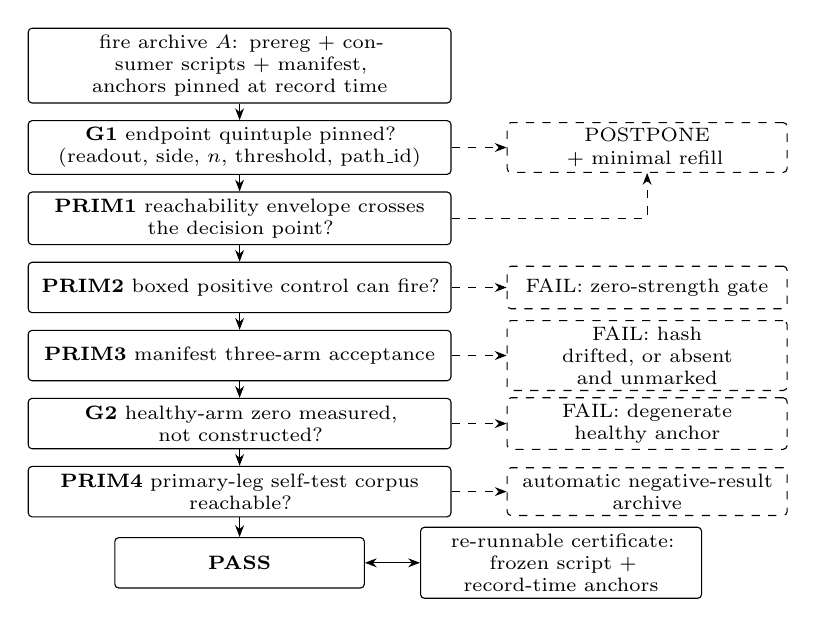
\begin{tikzpicture}[
  font=\scriptsize,
  box/.style={draw,rounded corners=1.4pt,align=center,inner sep=2.4pt,
              minimum height=6.4mm,text width=52mm},
  outlet/.style={draw,dashed,rounded corners=1.4pt,align=center,inner sep=2.2pt,
              minimum height=5.4mm,text width=34mm},
  cert/.style={draw,rounded corners=1.4pt,align=center,inner sep=2.4pt,
               minimum height=6.4mm,text width=34mm},
  flow/.style={-{Stealth[length=1.5mm]}},
  side/.style={-{Stealth[length=1.5mm]},dashed}]

\node[box] (a) {fire archive $A$: prereg $+$ consumer scripts $+$ manifest,\\
                anchors pinned at record time};
\node[box,below=2.1mm of a] (g1) {\textbf{G1} endpoint quintuple pinned?\\
                (readout, side, $n$, threshold, path\_id)};
\node[box,below=2.1mm of g1] (p1) {\textbf{PRIM1} reachability envelope crosses\\
                the decision point?};
\node[box,below=2.1mm of p1] (p2) {\textbf{PRIM2} boxed positive control can fire?};
\node[box,below=2.1mm of p2] (p3) {\textbf{PRIM3} manifest three-arm acceptance};
\node[box,below=2.1mm of p3] (g2) {\textbf{G2} healthy-arm zero measured,\\
                not constructed?};
\node[box,below=2.1mm of g2] (p4) {\textbf{PRIM4} primary-leg self-test corpus\\
                reachable?};
\node[box,below=2.5mm of p4,text width=30mm] (pass) {\textbf{PASS}};

\node[outlet,right=7mm of g1] (post) {POSTPONE\\ $+$ minimal refill};
\node[outlet,right=7mm of p2] (f2) {FAIL: zero-strength gate};
\node[outlet,right=7mm of p3] (f3) {FAIL: hash drifted, or absent\\ and unmarked};
\node[outlet,right=7mm of g2] (f4) {FAIL: degenerate\\ healthy anchor};
\node[outlet,right=7mm of p4] (f5) {automatic negative-result\\ archive};
\node[cert,right=7mm of pass] (cert) {re-runnable certificate:\\
                frozen script $+$ record-time anchors};

\draw[flow] (a) -- (g1);
\draw[flow] (g1) -- (p1);
\draw[flow] (p1) -- (p2);
\draw[flow] (p2) -- (p3);
\draw[flow] (p3) -- (g2);
\draw[flow] (g2) -- (p4);
\draw[flow] (p4) -- (pass);
\draw[side] (g1) -- (post);
% PRIM1 also exits to POSTPONE; route it below the POSTPONE box and enter from the
% bottom edge, because the earlier "|- (post.south east)" path ran along the inside of
% that box's bottom border and parked its arrowhead on the box corner.
\draw[side] (p1.east) -- ++(4mm,0) -| (post.south);
\draw[side] (p2) -- (f2);
\draw[side] (p3) -- (f3);
\draw[side] (g2) -- (f4);
\draw[side] (p4) -- (f5);
\draw[{Stealth[length=1.5mm]}-{Stealth[length=1.5mm]}] (pass) -- (cert);
\end{tikzpicture}
\caption{Schematic of the AUDIT-GATE decision path; the figure carries no quantitative
content. Solid arrows are the operability chain, dashed arrows are terminating verdicts.
Every terminal verdict, PASS included, is emitted together with a re-runnable
certificate, and POSTPONE carries the minimal refill that would make the endpoint
decidable. Symbols match Section~\ref{sec:framework}; the observer-round parameter of
Section~\ref{sec:binding} ($K=2$ by default) applies to consumption verdicts rather than
to the chain drawn here.}
\label{fig:pipeline}
\end{figure}

\begin{table}[H]
\caption{The registered verdict-state map (\texttt{analysis/VERDICT\_STATE\_MAP\_R41.json},
sha16 \texttt{e892db517faebfba}): all $26$ unit strings the checkers can emit, with the
state tally $13$ FAIL, $9$ PASS and $4$ POSTPONE. The $3$ strings of the second codomain, which are verdicts about an audit run
rather than about an archive, are Table~\ref{tab:statemapgroup}. Tags: \emph{live} $=$
emitted on the audited corpus of
Table~\ref{tab:ledger}; \emph{fixture} $=$ exercised only on a synthetic archive;
\emph{diagnostic} $=$ printable but never archived as a case verdict; \emph{historical} $=$
superseded; \emph{edition-gated} $=$ emitted by an earlier edition of the runner only. Every
POSTPONE row is tagged \emph{fixture}, \emph{diagnostic} or \emph{historical}, which is the
coverage gap of Section~\ref{sec:fixtures} in its most compact form.}
\label{tab:statemap}
\centering
\scriptsize
\setlength{\tabcolsep}{3pt}
\begin{tabular}{@{}L{118pt} c L{40pt} L{175pt}@{}}
\toprule
Machine string & State & Case & Predicate, and how it is exercised \\
\midrule
\path{PASS_OPERATIONAL} & PASS & F4
  & all registered computors present and non-empty \emph{(live)} \\
\path{PASS_OPERATIONAL_EXTERNAL_CANDIDATE} & PASS & A4
  & four lineage pins match sha16, positive gate passes and is usable, fail arm all-FAIL
    and not usable \emph{(live)} \\
\path{PASS} & PASS & D1 units
  & the per-unit acceptance criteria of the D1 runner \emph{(live)} \\
\path{FINAL_FIRE_LANDED} & PASS & F5 amend.
  & amendment spec name pinned in the job file and verdict file present; emitted behind the
    \path{__r29_pin__} marker \emph{(live)} \\
\path{REACHABLE} & PASS & F1
  & at least one computor hit \emph{(diagnostic)} \\
\path{PATCHED_OK} & PASS & F2
  & the empty-set fallback has been patched \emph{(diagnostic)} \\
\path{TELESCOPE_CLOSED} & PASS & F6
  & the telescope predicate is false, i.e.\ the repair landed \emph{(fixture)} \\
\path{ANCHOR_BYTE_STABLE} & PASS & PTSD-4
  & PRIM3 anchor state 1 of 5: the recomputed digest equals the record-time pin
    \emph{(live: 20 of 22 pins of Figure~\ref{fig:replay}; also PTSD-4)} \\
\path{PASS_ANCHOR_DRIFT_EXPLAINED} & PASS & PTSD-5
  & PRIM3 anchor state 2 of 5: digest differs, a cause is registered for that path, and the
    unit verdict recomputes unchanged \emph{(live: the 2 remaining pins; also PTSD-5)} \\
\addlinespace[2pt]
\path{FAIL_MECHANICALLY_UNREACHABLE} & FAIL & F1
  & the registered readout has zero computor hits in every consumer script \emph{(live)} \\
\path{FAIL_EMPTY_SET_PASSED_GATE} & FAIL & F2
  & an empty-denominator fallback (zero total, rate falls back to $1.0$) is present and
    unpatched \emph{(live)} \\
\path{FAIL_ABSENT_UNMARKED} & FAIL & F2, F5
  & a referenced artifact is absent and carries no ABSENT marker \emph{(live)} \\
\path{FAIL_ABSENT_UNMARKED_4_OF_5} & FAIL & F3
  & at least four of five recorded consumer paths absent at their recorded locations, with
    no ABSENT marker at record time \emph{(live)} \\
\path{FAIL_TELESCOPE} & FAIL & F6
  & $T(p)$ of Section~\ref{sec:prim5}: both transition branches occur in one tool source
    \emph{(live)} \\
\path{FAIL_DEGENERATE_HEALTHY_ANCHOR} & FAIL & seat F
  & the healthy arm's zero holds by construction and the threshold's only real anchor is a
    mismatched-path arm \emph{(live)} \\
\path{FAIL_SPEC_DRIFT} & FAIL & F5 legacy
  & the legacy spec name is no longer pinned in the job file after an authorised rename
    \emph{(live, informational: the ledger records this as a pointer to the amendment, not
    as an audited-archive FAIL, which is why the legacy invocation's exit code is not
    treated as a verdict)} \\
\path{FAIL_MISSING_COMPUTOR} & FAIL & F4
  & any registered computor missing or empty; the mirror of F4's pass \emph{(fixture)} \\
\path{FAIL_LINEAGE_DRIFT} & FAIL & A4
  & a lineage pin's sha16 drifted, or positive/fail-arm content drifted \emph{(fixture)} \\
\path{FAIL_FINAL_UNANCHORED} & FAIL & F5 amend.
  & the amendment spec name is not pinned, or the verdict file is absent \emph{(fixture)} \\
\path{FAIL_NULL_PRIMARY_LEG} & FAIL & PTSD-3
  & PRIM4: the registered primary self-test leg has zero scorable rows, so the archiving
    verdict holds and relabelling the leg is forbidden \emph{(fixture; zero live
    occurrences)} \\
\path{FAIL_ANCHOR_DRIFT_UNEXPLAINED} & FAIL & PTSD-6
  & PRIM3 anchor state 3 of 5: digest differs and no cause is registered for that path
    \emph{(fixture; also the mutation control of Section~\ref{sec:replay})} \\
\path{FAIL_NO_ROPE_ARM} & FAIL & seat H
  & the registered rope arm is absent or under-$n$ in the smoke report \emph{(edition-gated:
    emitted by the runner edition of the first run, whose group-level misclassification is
    Table~\ref{tab:preregdiff}; the current frozen edition's seat-H unit passes)} \\
\addlinespace[2pt]
\path{POSTPONE} & POSTPONE & D1 unit; fixtures
  & a unit-level exception, or registration incompleteness; always carries the minimal
    refill \emph{(fixture; zero occurrences on the live corpus)} \\
\path{STALE_NOT_REPRODUCED} & POSTPONE & F3
  & fewer than four stale paths absent, so either the archive changed or the ledger is
    stale --- and by PRIM3 the second reading is a self-FAIL of this ledger
    \emph{(diagnostic)} \\
\path{POSTPONE_ANCHOR_ABSENT_MARKED} & POSTPONE & PTSD-7
  & PRIM3 anchor state 4 of 5: the pinned path is absent and an ABSENT marker was written at
    record time; the refill is the whole file \emph{(fixture)} \\
\path{TBD_PROVISIONAL} & POSTPONE & F5 ledger
  & an in-flight fire attempt pending an authorised landing; a ledger state rather than a
    checker output at this round \emph{(historical, superseded by the r29 amendment)} \\
\bottomrule
\end{tabular}
\end{table}

Table~\ref{tab:statemap} is the whole of the map that PRIM5
(Section~\ref{sec:prim5}) requires, transcribed from the registered file. Reading it is the
only way to check Table~\ref{tab:ledger} without running the projection script, and it is
also the place where the framework's own coverage is visible: the right-hand tags say,
string by string, whether the live corpus ever emitted it. Four conventions are worth
stating. The bare string \path{PASS} is a verdict string as well as a state name, so the
identity map on it is registered explicitly rather than assumed. The \path{__r29_pin__}
prefix is stripped before lookup, so it needs no entries of its own. A string tagged
\emph{diagnostic} is one a checker can print but the ledger never archives as a case verdict;
it is registered anyway, because PRIM5 closes the domain over what the checkers \emph{can}
emit, not over what they happened to emit. And the map has a second codomain,
Table~\ref{tab:statemapgroup}: those three strings are verdicts about an audit run, they are
produced by a different rule from the unit strings, and the one time we conflated the two
levels the result was the false kill of Table~\ref{tab:preregdiff}. Where a row names a
fixture, the identifier is the one the runner emits, since that is the executed artifact.

\begin{table}[H]
\caption{The second codomain of the same registered map: the $3$ group strings
($2$ FAIL, $1$ PASS), which are
verdicts about an audit \emph{run} rather than about an archive and are produced by a
different rule from the unit strings of Table~\ref{tab:statemap}. Keeping the two codomains
in separate blocks is not cosmetic: the one time we conflated the levels, the result was the
false kill of Table~\ref{tab:preregdiff}.}
\label{tab:statemapgroup}
\centering
\scriptsize
\setlength{\tabcolsep}{3pt}
\begin{tabular}{@{}L{118pt} c L{40pt} L{175pt}@{}}
\toprule
Machine string & State & Case & Predicate, and how it is exercised \\
\midrule
\path{EXECUTION_VALID} & PASS & D1 group
  & no unit string is unmapped and the projected multiset is not one repeated state, i.e.\
    the audit ran and discriminated \emph{(live; renamed from the legacy
    \path{AUDIT_EXECUTION_PASS} label without changing semantics)} \\
\path{FAIL_VACUOUS_STATES} & FAIL & D1 group
  & the projected unit multiset collapses to a single state, so the audit did not
    discriminate on this corpus \emph{(synthetic all-identical multiset, plus one recorded
    historical instance: the first run under the first-edition rule,
    Table~\ref{tab:preregdiff} --- that instance is recorded, not recomputable, the
    pre-fix edition being absent from disk, Section~\ref{sec:operable})} \\
\path{FAIL_UNMAPPED_VERDICT} & FAIL & D1 group
  & some unit string has no entry here and no prefix rule applies; this is the enforcement
    mechanism of rule (ii) \emph{(never fired on the frozen report)} \\
\bottomrule
\end{tabular}
\end{table}

\section{Synthetic fixtures and the pre-registration diff}
\label{app:fixtures}

Table~\ref{tab:fixtures} is the per-fixture record behind Section~\ref{sec:fixtures}, and
Table~\ref{tab:preregdiff} is the pre-registration diff that Section~\ref{sec:operable}
commits us to. The two belong together: the first shows the framework's unexercised clauses
firing on inputs we built, and the second shows the one occasion on which the framework's own
gate had to be changed after seeing an observation.

The authored fixtures cover the branches absent from the live corpus. One tests an
incomplete G1 registration, one searches the non-crossing PRIM1 envelope for its refill,
and one exercises an unreachable primary leg. The remaining fixtures enumerate PRIM3 as a
total function of path presence, digest equality, a recorded cause, and an ABSENT marker.
Each archive carries one injected defect and an expected verdict; the runner derives the
observed verdict and exits non-zero on disagreement. These are positive controls for
mechanical operability, not estimates of performance on natural archives.

{
\setlength{\tabcolsep}{3pt}
\setlength{\LTcapwidth}{\linewidth}
\begin{longtable}{@{}>{\scriptsize}l Q{112pt} Q{128pt} Q{109pt}@{}}
\caption{The eight synthetic defect-injected fixtures. Each injects exactly one defect and
carries its expected verdict as a registered field, so the runner
(\texttt{code/audit\_gate\_fixtures.py}) compares rather than asserts; it recomputes each verdict
from first principles, including searching for $n^{\star}$ rather than looking it up. PTSD-1
and PTSD-2 POSTPONE under G1's missing-field rule. PTSD-4
to PTSD-8 are one archive per row of the five-state PRIM3 anchor enumeration, and the runner
also checks that the enumeration is total. Expected and observed verdicts match on all eight
rows, and the run uses no GPU. Report:
\texttt{analysis/FIXTURE\_RESULTS\_R41.json}, sha16 \texttt{963a9795cfa42867}.}
\label{tab:fixtures}\\
\toprule
ID & Injected defect & Verdict (expected ${}={}$ observed) & Minimal refill \\
\midrule
\endfirsthead
\multicolumn{4}{@{}l}{\scriptsize\tablename~\thetable\ (continued)}\\
\toprule
ID & Injected defect & Verdict (expected ${}={}$ observed) & Minimal refill \\
\midrule
\endhead
\midrule
\multicolumn{4}{r@{}}{\scriptsize Continued on next page}\\
\endfoot
\bottomrule
\endlastfoot
PTSD-1 & G1 quintuple registers \texttt{readout}, \texttt{side}, $n$ but omits
  \texttt{threshold} and \texttt{path\_id} & \path{POSTPONE}
  & the two named missing fields \\
\addlinespace[2pt]
PTSD-2 & PRIM1 envelope does not cross: $k=0$, $n=40$, \textsc{lo} side, $\theta=0.03$,
  so $U=0.0881$ & \path{POSTPONE}
  & $82$ observation rows, reaching $n^{\star}=122$ \\
\addlinespace[2pt]
PTSD-3 & PRIM4 primary self-test leg has zero scorable rows and is relabelled as a
  sensitivity analysis & \path{FAIL_NULL_PRIMARY_LEG}
  & none: the archiving verdict holds automatically \\
\addlinespace[3pt]
\multicolumn{4}{@{}L{\linewidth}@{}}{\scriptsize\emph{PRIM3 record-time anchor enumeration, one fixture per state
  (present?, digest equal?, cause recorded?, ABSENT marker?):}} \\
\addlinespace[1pt]
PTSD-4 & state 1 of 5: pinned artifact present, digest equals the record-time pin
  & \path{ANCHOR_BYTE_STABLE} & none \\
\addlinespace[2pt]
PTSD-5 & state 2 of 5: present, digest differs, a cause is recorded for that path
  & \path{PASS_ANCHOR_DRIFT_EXPLAINED} & none; the cause entry is the obligation \\
\addlinespace[2pt]
PTSD-6 & state 3 of 5: present, digest differs, no cause recorded
  & \path{FAIL_ANCHOR_DRIFT_UNEXPLAINED}
  & record a checkable cause, or the state stands \\
\addlinespace[2pt]
PTSD-7 & state 4 of 5: pinned path absent, ABSENT marker written at record time
  & \path{POSTPONE_ANCHOR_ABSENT_MARKED}
  & re-materialise the file at its recorded path (quantum: whole file) \\
\addlinespace[2pt]
PTSD-8 & state 5 of 5: pinned path absent, no marker
  & \path{FAIL_ABSENT_UNMARKED}
  & none: the FAIL stands until the file or a record-time marker exists \\
\end{longtable}
}

{
\setlength{\tabcolsep}{3pt}
\setlength{\LTcapwidth}{\linewidth}
\begin{longtable}{@{}Q{72pt} Q{102pt} Q{102pt} Q{55pt} Q{42pt}@{}}
\caption{Post-observation amendments to this framework's own registered objects, disclosed
as findings of the construction, not as defects (Section~\ref{sec:operable}). Three are design-level (gate and
definition editions); the fourth is the external-review repair disclosed in
Section~\ref{sec:g2}. On the gate row the three rule editions are separated explicitly,
because an earlier version of this note labelled the first-run implementation's semantics
as the registered one --- it was not: the registered predicate never counted ``any FAIL as
collapse'', and the amendment moved the shipped rule \emph{toward} the pre-registration.
``Re-executable'' asks whether the semantics named in that row can still be run from bytes
on this disk today; one row answers no, and that row is this note's one recorded,
non-recomputable verdict (Section~\ref{sec:operable}).}
\label{tab:preregdiff}\\
\toprule
Object and trigger & Superseded semantics & Current semantics & Where filed &
Re-exec. \\
\midrule
\endfirsthead
\multicolumn{5}{@{}l}{\scriptsize\tablename~\thetable\ (continued)}\\
\toprule
Object and trigger & Superseded semantics & Current semantics & Where filed &
Re-exec. \\
\midrule
\endhead
\midrule
\multicolumn{5}{r@{}}{\scriptsize Continued on next page}\\
\endfoot
\bottomrule
\endlastfoot
Group-gate diversity criterion; trigger: the first run's legitimate
\path{FAIL_NO_ROPE_ARM} on the seat-H unit was read by the first-run code as a group-level collapse
  & \textbf{v1, first-run code} (\emph{not} the registered text): any unit FAIL is read as
    a collapsed verdict set, hence group \path{FAIL_VACUOUS_STATES}.
    \textbf{v3, registered} (prereg \S3, \emph{never changed}): the state set is neither
    all-PASS nor all-FAIL nor all-POSTPONE --- v3 already accepted the first run's
    multiset, so v1 was inconsistent with the prereg and the amendments moved
    \emph{toward} it
  & \textbf{v2} (R31): a G2 caveat is a separate bucket counted as a detection; an
    ordinary FAIL still counts toward collapse. \textbf{v2b} (R42, current): v2 plus
    \emph{any} FAIL-family string counts as a distinct observed state in the second
    disjunct --- the reading v3 had all along
  & ``correction (R31)'' of \path{audit_gate_d1_summary.md}; the prereg's post-run
    amendment note; v2/v2b/v3 executable in \path{code/group_state_rule.py}
  & \textbf{v1: no}; v2, v2b, v3: yes \\
\addlinespace[3pt]
The registered verdict-state map, v1 to v2
  & the map registered the strings the two panels had emitted; the PRIM4 and anchor-state
    strings had no entry, so the projection script would have exited non-zero on them
  & every string any checker of this note can emit is registered, each tagged with how it
    was exercised (live, fixture, diagnostic, historical, edition-gated)
  & the \path{v2_changes} block inside the map file itself & yes \\
\addlinespace[3pt]
PRIM3, from three arms to a five-state enumeration
  & ``exactly one of three arms applies'': present with matching hash (PASS), present with
    drifted hash and no recorded cause (FAIL), absent without a marker (FAIL)
  & the same decision as a total function of four record-time facts, with five reachable
    states; the two added are drift-with-a-recorded-cause (PASS) and absent-with-a-marker
    (POSTPONE). Two anchors of our own certificate fall in the gap; the certificate check
    prints the tally with and without the cause registry, and no unit verdict differs under
    that anchor-state toggle (Section~\ref{sec:replay})
  & \path{code/prim3_anchor_states.py} and the state-map file & yes \\
\addlinespace[3pt]
G2 and three Panel-B predicates, from constants to predicates (external review, R42)
  & the seat-F verdict was an unconditional assignment while its inputs were read from keys
    absent from the cell file (every read \texttt{None}, none entering a condition); the
    seat-C/seat-E/seat-G acceptance conjunctions were near-tautological (one \texttt{RESOLVED} token;
    a substring matching ``harm''; two-word presence)
  & G2 is a predicate over the audited cell's own fields (\texttt{bit\_exact} true or
    \texttt{max\_max}${}=0$ on the healthy arm); seat C verifies a registered per-slot
    manifest; seat E requires the bound string plus an explicit three-arm mention; seat G requires
    the trial id and the pinned spec name in the job file. At the R42 repair point, unit
    verdicts were unchanged on all seven units
  & \path{code/run_audit_gate_d1.py} R42 edition and the
    \path{judge_version_drift} field of the R42 projection; the R31 frozen certificate is
    untouched & yes \\
\end{longtable}
}

\section{Internal checks on our own checkers}
\label{app:internal}

Three measurements in this appendix are checks of the auditing code rather than of any audited
archive. They are grouped here because they share one limitation: we wrote both sides.

\paragraph{The two group-rule editions are incomparable.}
Section~\ref{sec:prim5} states the group readout as a registered predicate, and the decisive
cell shipped a different rule. Their complete disagreement counts and smallest witnesses are
in Table~\ref{tab:rulediff}; neither rule refines the other.

\begin{table}[H]
\caption{Bidirectional group-rule disagreement over the registered verdict-multiset domain.
Reading: neither edition contains the other.}
\label{tab:rulediff}
\centering
\scriptsize
\setlength{\tabcolsep}{3pt}
\begin{tabular}{@{}L{70pt} L{70pt} c L{210pt}@{}}
\toprule
Accepted by & Rejected by & Count & Smallest witness \\
\midrule
Registered predicate & Shipped rule & $75$
  & six PASS units plus one \path{FAIL_NO_ROPE_ARM} \\
Shipped rule & Registered predicate & $21$
  & six \path{FAIL} units plus one \path{FAIL_DEGENERATE_HEALTHY_ANCHOR} \\
\bottomrule
\end{tabular}
\end{table}

The first witness is the R31 misfire pattern minus its G2 caveat, showing that the correction
of Section~\ref{sec:operable} rescued only multisets containing a G2 verdict and left the
shipped rule inconsistent with the registered text elsewhere. The second is an all-FAIL
multiset that the pre-registration excludes as a vacuum and the shipped rule passes. The
multiset our corpus actually produced lies outside both disagreement sets, so no verdict
reported in this note changes under either rule --- which is a fact about our corpus and not
a defence of the rule.

\paragraph{A second implementation of five checks.}
\path{code/audit_gate_second_impl.py} re-implements five checks from their written
specifications by deliberately different means: the string projection by longest-literal
matching over the map file rather than by dictionary lookup; the PRIM3 anchor states by an
explicit $16$-row lookup table rather than by nested conditions; the Clopper--Pearson
zero-column limit by bisecting the exact binomial tail rather than by the closed form of
Section~\ref{sec:prims}; the fixture verdicts by one purpose-written reader per fixture; and
the group predicate by a pairwise diversity test rather than by the shipped rule. The two
implementations agree on every unit, every truth-table row, every fixture and the group
readout. The only numerical difference is $|U_{\text{closed}}(40)-U_{\text{bisect}}(40)| =
4.4\times10^{-16}$, with both routes returning $n^{\star}=122$ and a refill of $82$ rows. This
catches only errors that survive one implementation and not the other; it is not independence.

\paragraph{Design numbers of the registered calibration cell.}
The bounds that fix the design of Section~\ref{sec:falsification}'s calibration cell are
computed by \path{code/cp_design_numbers.py} rather than asserted; the aligned detection and
false-alarm designs are Tables~\ref{tab:cpdetection} and~\ref{tab:cpfalsealarm}. The first pass
is a pilot that reports intervals only, while the confirmatory pass requires $36$ archives per
family. The pre-registration freezes the defect-free stratum at $60$ with a one-fire allowance
and forbids growing it after fires are seen.

\begin{table}[H]
\caption{Per-family detection design under two-sided $95\%$ Clopper--Pearson intervals.}
\label{tab:cpdetection}
\centering
\small
\setlength{\tabcolsep}{6pt}
\begin{tabular}{@{}L{270pt}L{100pt}@{}}
\toprule
Quantity & Registered value \\
\midrule
Lower bound at $10/10$ & $0.6915$ \\
Detection criterion & $0.90$ \\
Bound at $n=35$ (last value below the criterion) & $0.89997$ \\
First $n$ at which the bound crosses the criterion & $36$ \\
\bottomrule
\end{tabular}
\end{table}

\begin{table}[H]
\caption{Pooled defect-free false-alarm design at $n=60$. Reading: the registered upper
bound $0.10$ tolerates exactly one fire; tolerating two requires $n=70$, and tolerating three
requires $n=85$.}
\label{tab:cpfalsealarm}
\centering
\small
\setlength{\tabcolsep}{6pt}
\begin{tabular}{@{}L{270pt}L{100pt}@{}}
\toprule
Fires & Clopper--Pearson upper bound \\
\midrule
$0$ & $0.0596$ \\
$1$ & $0.0894$ \\
$2$ & $0.1153$ \\
\bottomrule
\end{tabular}
\end{table}

\section{Remaining delineation axes and inherited anti-patterns}
\label{app:delta}

\paragraph{Axes D4 and D5.}
\emph{D4, output type}: the neighbour ships a gate script plus a written list of
anti-patterns, that is, governance experience; this note ships a primitive layer, a
variable-rate fan-in ledger whose FAIL channel is demonstrated, and the methods note
itself. \emph{D5, relation to the model}: the neighbour serves the readout layer of one
inference stack and has no fine-tuning or checkpoint-phase concept, whereas AUDIT-GATE is
object-agnostic, and the archives it audits in Table~\ref{tab:ledger} include fine-tuning
differentials, checkpoint-margin calibration, evaluation-distortion probes and pure CPU
pipelines. Overlap self-assessment, stated plainly: zero at the claim layer, roughly a
quarter at the level of method vocabulary, since ``gate'', ``control'' and ``envelope''
are statistical common property.

\paragraph{The six inherited anti-patterns.}
Reused, not reproved: (i) an empty set must fail a gate rather than pass it; (ii) a
rate-only test is blind to direction; (iii) a run identifier must be a field, not a
directory name; (iv) a truncated output is not a wrong answer; (v) short-sample behaviour
does not certify long-generation behaviour; (vi) static inspection cannot see a runtime
crash. PRIM2 and PRIM3 are the mechanical forms of (i) and (iii); (iv) and (v) survive as
reasons why a readout-layer gate remains necessary alongside this one.

\paragraph{Two clauses added from the in-run review pipeline.}
The list continues with two clauses that reached us as review output on other seats' gates
rather than as our own findings; they are stated here as normative clauses of the audit, and
their falsification conditions are in Section~\ref{sec:falsification}.

\emph{(vii)} A structural reachability precheck is a
\emph{sufficient-rejection, necessary-but-not-sufficient-admission} gate: a pre-registered
upper bound computed before ordering --- for instance $\max(b+c)$ for a McNemar-framed test,
or a permutation design's $p_{\mathrm{floor}}$ together with a tolerance table --- proves only
that the test is not mechanically unanswerable. It does not prove that admission was correct.
A positive control that purports to demonstrate no false kill must itself survive clause
(viii); otherwise its pass records a false admission.

\emph{(viii)} Any reference arm or control fixture whose \emph{load-bearing numeric fields}
are byte-identical to another arm's, beyond the metadata divergence one would expect, FAILs
the audit. The converse trap is the reason the clause is written on fields rather than on
files: two arms with distinct bytes and distinct inodes can still carry the same measurement
--- in the case that prompted this clause, a run's \texttt{always} and \texttt{never}
reference pair agreed byte-for-byte in $20$ of $22$ top-level fields --- so the audit must
compare numeric payloads field by field, and its object must extend past the outputs
directory to every artifact consumed downstream, including probe and perturbation copies,
pre-gate analyser outputs, and any record that references those cells. Byte-level and
inode-level checks are blind to exactly this failure.

\paragraph{Provenance of clauses (vii) and (viii).}
Neither clause is ours, and both were revised at least once before being admitted here, so we
record the chain rather than the conclusion alone. Clause (vii) descends from a reachability
precheck note whose first version over-claimed the mechanism and was corrected by a teacher
review; clause (viii) descends from a fault-reconciliation record on another seat, which
established that the defect's real channel was a wiring equivalence between two reference arms
rather than a directory copy, and that hash- and inode-level auditing is blind to it. A
separate seat's own v2 correction retired a quantitative prior we had earlier attached to
clause (vii) --- an ``about a quarter of cells are unreachable'' figure that its authors
withdrew --- and we removed the number rather than restating it. The provenance records that
carry this chain are organised in Table~\ref{tab:clauseprov}; the baseline and its addendum
are two editions of the local clause record.

\begin{table}[H]
\caption{Read-only provenance chain for clauses (vii) and (viii). The two sha16 values pin
the local draft editions; the neighbour records are cited at their run-tree locations.}
\label{tab:clauseprov}
\centering
\scriptsize
\setlength{\tabcolsep}{3pt}
\begin{tabular}{@{}L{260pt} L{120pt}@{}}
\toprule
Record & Role \\
\midrule
Fault-reconciliation memo of neighbour seat E (anonymized; retained in the run tree)
  & fault reconciliation behind clause (viii) \\
Corrected reachability analysis of neighbour seat C (anonymized; retained in the run tree)
  & corrected reachability analysis \\
Registered source design of neighbour seat C (anonymized; retained in the run tree)
  & registered source design \\
Local baseline clause draft (sha16 \path{2ed57f6b51b6ce2c})
  & baseline clause draft \\
Local superseding addendum (sha16 \path{5ca2e2d3ade43a7d})
  & superseding addendum \\
\bottomrule
\end{tabular}
\end{table}

We hold none of the first three; they are cited as located, read-only
neighbour records, and the numbers we dropped on their authority are dropped rather than
re-derived.

\section{Per-unit endpoint registration in the decisive cell}
\label{app:g1}

The complete G1 rule is
$e=(\text{readout},\text{side},n,\text{threshold},\text{path\_id})$.
A missing field makes the endpoint unregistered and returns POSTPONE with the smallest
missing-field or observation-row refill that restores decidability. The path identity
fingerprints the decoding or serving route, weight/configuration state, and readout parser
or grader; a threshold is valid only within that identity. These last two fields were added
after adjudication showed that sample count and threshold alone underdetermine the
observation path.

Two tiers must be distinguished. In the frozen R31--R42 tier, the G1 quintuples and G2
answers are auditor transcriptions, not mechanical extractions: per-unit constants written
after reading each archive. The frozen ``$5/5$'' therefore counts transcribed fields, not
fields proved present. The current tier instead uses one parser per archive schema
(\path{code/audit_gate_g1_extractor.py} and
\path{code/audit_gate_g1_parsers.py}); unparseable or contradicted fields degrade to
POSTPONE under G1's missing-field rule. Five units extract fully; seat C POSTPONEs because
G2 is not mechanically parseable, and seat H POSTPONEs because its threshold is not.
Eleven delete/mutate ablations plus constant-grep and identity controls pass in
\path{experiments/results/audit_gate_d1/g1_extractor_ablation_log.json}. The runner consumes
these evidence records directly, making the current sidecar the mechanical-extraction tier
while the frozen report remains the transcription tier.

\begin{table}[htbp]
\caption{Two provenance tiers of the decisive cell. Panel A is the current mechanical-
extraction tier, with current-verdict tally $3$ PASS, $2$ FAIL, $2$ POSTPONE; Panel B is
the frozen auditor-transcription record, tally $6$ PASS, $1$ FAIL, $0$ POSTPONE. Frozen
G1/G2 fields are auditor transcriptions, not mechanical extractions.}
\label{tab:g1units}
\centering
\scriptsize
\setlength{\tabcolsep}{4pt}
% Verdict column is 128pt so that FAIL_DEGENERATE_HEALTHY_ANCHOR (126.0pt at \scriptsize)
% stays on one line; the width comes out of the Unit column, whose widest key is 79.8pt.
\begin{tabular}{@{}L{84pt} L{128pt} c c c@{}}
\toprule
\multicolumn{5}{@{}l}{\emph{Panel A: current mechanical-extraction tier}}\\
Unit & Current verdict & G1 mech. & G2 mech. & Pins \\
\midrule
\path{D_A4_healthgate}$^\star$ & \path{PASS} & 5/5 & yes & 4 \\
\path{C_exit_package_R42} & \path{POSTPONE} (G2) & 5/5 & not parseable & 4 \\
\path{E_R33_threearm} & \path{FAIL} & 5/5 & yes & 3 \\
\path{F_r42_samepath} & \path{FAIL_DEGENERATE_HEALTHY_ANCHOR} & 5/5 & yes & 4 \\
\path{G_fb2_v3_r120} & \path{PASS} & 5/5 & yes & 2 \\
\path{H_r7_conject_front} & \path{POSTPONE} (threshold) & 4/5 & yes & 3 \\
\path{A_r7_strict_corpus} & \path{PASS} & 5/5 & yes & 2 \\
\midrule
\multicolumn{5}{@{}l}{\emph{Panel B: frozen R31--R42 auditor-transcription record}}\\
Unit & Frozen verdict & G1 transcribed & G2 answered & Pins \\
\midrule
\path{D_A4_healthgate}$^\star$ & \path{PASS} & 5/5 & yes & 4 \\
\path{C_exit_package_R42} & \path{PASS} & 5/5 & yes & 4 \\
\path{E_R33_threearm} & \path{PASS} & 5/5 & yes & 3 \\
\path{F_r42_samepath} & \path{FAIL_DEGENERATE_HEALTHY_ANCHOR} & 5/5 & mech.\ (current) & 4 \\
\path{G_fb2_v3_r120} & \path{PASS} & 5/5 & yes & 2 \\
\path{H_r7_conject_front} & \path{PASS} & 5/5 & yes & 3 \\
\path{A_r7_strict_corpus} & \path{PASS} & 5/5 & yes & 2 \\
\bottomrule
\end{tabular}
\end{table}

\section{Canonical pin}
\label{app:pin}

This appendix is the single canonical statement of the audit claim and supersedes every
historical tier for current-verdict reporting. The certificate verifier attests this pin:
the canonical checker, its recorded input pins, the current mechanical-extraction verdict,
the frozen verdict retained as history, and the replay interface. The decisive-cell current
tally is $3$ PASS, $2$ FAIL, $2$ POSTPONE; the frozen tally is $6$ PASS, $1$ FAIL, $0$
POSTPONE. Table~\ref{tab:pin} is therefore single-valued with Table~\ref{tab:g1units} and
the tier caveats in Table~\ref{tab:ledger}.

{\setlength{\tabcolsep}{2pt}
\begin{longtable}{@{}Q{92pt} Q{68pt} Q{78pt} Q{78pt} Q{54pt}@{}}
\caption{Canonical pin: one row per decisive-cell unit and one block for the six-case
ledger. The checker and input descriptions identify the recorded evidence; current and
frozen verdicts are kept in separate columns.}\label{tab:pin}\\
\toprule
Unit & Checker sha16 & Input pins & Current verdict & Frozen verdict \\
\midrule
\endfirsthead
\multicolumn{5}{@{}l}{\scriptsize\tablename~\thetable\ (continued)}\\
\toprule Unit & Checker sha16 & Input pins & Current verdict & Frozen verdict \\
\midrule
\endhead
\midrule\multicolumn{5}{r@{}}{\scriptsize Continued on next page}\\
\endfoot
\bottomrule
\endlastfoot
\multicolumn{5}{@{}l}{\emph{Decisive cell; replay: \path{run_audit_gate_d1.sh}}}\\
\path{D_A4_healthgate}$^\star$ & \path{9286a81b3f4c9f7a} & owner-gate lineage & PASS & PASS \\
\path{C_exit_package_R42} & \path{9286a81b3f4c9f7a} & per-slot manifest & POSTPONE (G2) & PASS \\
\path{E_R33_threearm} & \path{9286a81b3f4c9f7a} & live-archive cell records & FAIL & PASS \\
\path{F_r42_samepath} & \path{9286a81b3f4c9f7a} & same-run cell records & FAIL (G2) & FAIL (G2) \\
\path{G_fb2_v3_r120} & \path{9286a81b3f4c9f7a} & owner-seat job pins & PASS & PASS \\
\path{H_r7_conject_front} & \path{9286a81b3f4c9f7a} & smoke-report records & POSTPONE (threshold) & PASS \\
\path{A_r7_strict_corpus} & \path{9286a81b3f4c9f7a} & corpus summaries & PASS & PASS \\
\midrule
\multicolumn{5}{@{}l}{\emph{Six-case ledger; replay: \path{python3 analysis/audit_gate.py}}}\\
F1--F6 and A4 & \path{0ed8657a6ab7dbf9} & Table~\ref{tab:anchors} pins
  & matches frozen ledger & matches frozen ledger \\
\end{longtable}}

Three scope clauses bind the pin. PASS certifies mechanical operability, not scientific
correctness. POSTPONE follows only from the audit's missing-field rule: seat C lacks a
mechanically established G2 answer and seat H lacks a certified threshold. Historical
transcriptions and replay snapshots remain in the ledger as the archaeological record,
not as competing current verdicts.

\section{Figure provenance}
\label{app:figures}

The four figures have three different provenances and we separate them, because a reader is
entitled to know which pixels came from data and which from a generator.

Figure~\ref{fig:pipeline} is a programmatic schematic drawn from the section it illustrates
and contains no quantitative content. Figures~\ref{fig:replay} and~\ref{fig:coverage} are
generated from on-disk artifacts by \path{code/make_replay_matrix.py} and
\path{code/make_coverage_matrix.py}; no value in either is entered by hand, and re-running the
scripts reproduces both, byte for byte --- each script suppresses the embedded creation
timestamp so that the figure PDFs are as reproducible as the JSON artifacts they are drawn
from.

Figure~\ref{fig:teaser} is a raster illustration produced with an image generator, and it is
the only generated asset in the manuscript. Its status is qualitative: it carries no quantitative value,
no measurement and no experimental outcome, and nothing in the paper's argument rests on it.
Three candidates were generated. The first was rejected on scientific-semantic grounds --- it
omitted the G2 check from the audit chain, which matters because G2 is the check that fires on
the one detection in Panel~B, and it showed the input archive with three components instead of
four. The second passed the element audit and was the prior adopted version. The third,
adopted here, preserves that version's semantics while making the PRIM5 projection an explicit
box between the raw machine string and the three mutually exclusive states. Audited element by
element against Section~\ref{sec:framework}, it shows the four archive objects, the six checks
in the order of Figure~\ref{fig:pipeline}, PRIM5 outside and after that stack, the three state
badges as its only outcomes, and a separate certificate path to a reviewer; no GPU appears,
and the illustration carries no measurement or experimental outcome. The prompts, tool,
candidates, semantic audits and adoption decisions are recorded in
\path{build/image_generation_record.json}. Two further facts belong there rather than in a caption. An
earlier round's attempt at this figure failed with a hard generator quota error, which is
logged in the same file; the quota had been restored by the time this version was drafted. And
the prompt asked for a specific image backend, but the tool exposed no backend
selector, so we record what was requested and do not claim to know which model rendered the
adopted asset.

\end{document}
